% lecture13.tex -- GENERATED by build_L13.py from L13_numbers.json; do not edit by hand.
\documentclass[10pt,aspectratio=169,t]{beamer}
% =============================================================================
% nn_preamble.tex -- shared Beamer preamble of Neural Networks and Deep Learning (NN)
% Used by every lecture: lectures/Lk/lecturek.tex does
%   \documentclass[10pt,aspectratio=169,t]{beamer}
%   % =============================================================================
% nn_preamble.tex -- shared Beamer preamble of Neural Networks and Deep Learning (NN)
% Used by every lecture: lectures/Lk/lecturek.tex does
%   \documentclass[10pt,aspectratio=169,t]{beamer}
%   % =============================================================================
% nn_preamble.tex -- shared Beamer preamble of Neural Networks and Deep Learning (NN)
% Used by every lecture: lectures/Lk/lecturek.tex does
%   \documentclass[10pt,aspectratio=169,t]{beamer}
%   \input{../common/nn_preamble}
%   \nnlecture{k}{Lecture title}
% Logos live in lectures/common/logos/, charts in lectures/Lk/charts/.
% Do NOT add \hfuzz / \vfuzz / \hbadness here: overfull boxes must be fixed, not hidden.
% =============================================================================

\usetheme{default}
\setbeamersize{text margin left=7mm, text margin right=7mm}

% ---------------------------------------------------------------- packages
\usepackage[utf8]{inputenc}
\usepackage[T1]{fontenc}
\usepackage{lmodern}
\usepackage{amsmath, amssymb}
\usepackage{mathtools}
\usepackage{bm}
\usepackage{tikz}
\usetikzlibrary{arrows.meta, positioning, calc, shapes.misc}
\usepackage{booktabs}
\usepackage{array}
\usepackage{graphicx}
\usepackage{colortbl}
\usepackage{xcolor}
\usepackage{multicol}
\hypersetup{colorlinks=true, linkcolor=MainBlue, urlcolor=MainBlue, citecolor=MainBlue}
\graphicspath{{../common/logos/}}   % charts are included with their language folder: charts/en/, charts/ro/

% ---------------------------------------------------------------- colours
\definecolor{MainBlue}{RGB}{26, 58, 110}
\definecolor{IDAred}{RGB}{205, 0, 0}
\definecolor{DarkGray}{RGB}{51, 51, 51}
\definecolor{FooterGray}{RGB}{100, 100, 100}
\definecolor{BlockGray}{RGB}{236, 238, 242}
\definecolor{KeynoteGray}{RGB}{218, 218, 218}
\definecolor{Crimson}{RGB}{190, 40, 50}
\definecolor{Forest}{RGB}{30, 110, 50}
\definecolor{Bitter}{RGB}{214, 150, 20}
% chart palette (same hex values and order as lectures/common/nn_plot.py SERIES)
\definecolor{Ser1}{HTML}{2A78D6}
\definecolor{Ser2}{HTML}{EB6834}
\definecolor{Ser3}{HTML}{1BAF7A}
\definecolor{Ser4}{HTML}{EDA100}
\definecolor{Ser5}{HTML}{E87BA4}
\definecolor{Ser6}{HTML}{008300}
\definecolor{Ser7}{HTML}{6250D6}
\definecolor{Ser8}{HTML}{E34948}

\setbeamertemplate{background}{%
  \begin{tikzpicture}[remember picture, overlay]
    \shade[shading=axis, shading angle=315, top color=white, bottom color=KeynoteGray]
      (current page.south west) rectangle (current page.north east);
  \end{tikzpicture}}
\setbeamercolor{background canvas}{bg=}
\setbeamercolor{structure}{fg=MainBlue}
\setbeamercolor{normal text}{fg=DarkGray}
\setbeamercolor{title}{fg=IDAred}
\setbeamercolor{frametitle}{fg=IDAred, bg=}
\setbeamercolor{block title}{bg=MainBlue, fg=white}
\setbeamercolor{block body}{bg=BlockGray, fg=DarkGray}
\setbeamercolor{block title alerted}{bg=Crimson, fg=white}
\setbeamercolor{block body alerted}{bg=Crimson!7, fg=DarkGray}
\setbeamercolor{block title example}{bg=Forest, fg=white}
\setbeamercolor{block body example}{bg=Forest!7, fg=DarkGray}
\setbeamercolor{item}{fg=MainBlue}
\setbeamerfont{frametitle}{size=\large, series=\bfseries}
\setbeamerfont{block title}{size=\small, series=\bfseries}
\setbeamertemplate{blocks}[rounded][shadow=false]
\setbeamertemplate{itemize item}{\color{MainBlue}$\boxdot$}
\setbeamertemplate{itemize subitem}{\color{MainBlue}\scriptsize$\blacktriangleright$}
% compact two-level lists: level 1 = main point, level 2 = details (no text outside bullets)
\setbeamerfont{itemize/enumerate subbody}{size=\footnotesize}
\setlength{\leftmargini}{1.1em}
\setlength{\leftmarginii}{1.1em}
\setbeamertemplate{itemize/enumerate body begin}{\setlength{\topsep}{0pt}\setlength{\partopsep}{0pt}\setlength{\parskip}{0pt}}
\setbeamertemplate{itemize/enumerate subbody begin}{\setlength{\topsep}{0pt}\setlength{\partopsep}{0pt}\setlength{\itemsep}{0pt}\vspace{-0.4ex}}

\setbeamertemplate{enumerate item}{\color{MainBlue}\insertenumlabel.}
\setlength{\leftmargini}{1.3em}
\setlength{\leftmarginii}{1.2em}
\setbeamertemplate{navigation symbols}{}
\setbeamertemplate{section in toc}{\color{MainBlue}$\blacktriangleright$~\inserttocsection}
\setbeamertemplate{caption}{\raggedright\insertcaption\par}
% frame subtitle = precise citation line under the claim title (Weron style)
\setbeamerfont{framesubtitle}{size=\footnotesize}
\setbeamercolor{framesubtitle}{fg=FooterGray}
% outline that reappears at every section with the current section highlighted
\setbeamertemplate{section in toc shaded}[default][35]
\setbeamertemplate{subsection in toc shaded}[default][35]
\setbeamertemplate{subsection in toc}{\leavevmode\leftskip=2.2em\color{DarkGray}\small\inserttocsubsection\par}
\AtBeginSection[]{{\begin{frame}{\txtoutline}\vspace{2mm}\small
  \tableofcontents[currentsection,hideothersubsections]\end{frame}}}

% ---------------------------------------------------------------- head and foot
\setbeamertemplate{headline}{%
  \vskip10pt%
  \hbox to \paperwidth{\hskip0.5cm%
    {\small\color{FooterGray}\renewcommand{\hyperlink}[2]{##2}\insertsectionhead}%
    \hfill\textcolor{FooterGray}{\small\insertframenumber}\hskip0.5cm}%
  \vskip4pt{\color{FooterGray}\hrule height 0.4pt}}
% footer as in the other courses (MFM, SFM): course name on the left, small sparkline on the right
\setbeamertemplate{footline}{%
  {\color{FooterGray}\hrule height 0.4pt}\vskip4pt%
  \hbox to \paperwidth{\hskip0.5cm%
    \textcolor{FooterGray}{\small\txtcourse}%
    \hfill\raisebox{-0.1em}{\begin{tikzpicture}[x=0.08em, y=0.08em, line width=0.4pt]
      \draw[FooterGray] (0,3) -- (1,4) -- (2,3.5) -- (3,5) -- (4,4) -- (5,6) -- (6,5.5) -- (7,4) -- (8,5) -- (9,7) -- (10,6) -- (11,5) -- (12,6.5) -- (13,8) -- (14,7) -- (15,6) -- (16,7.5) -- (17,9) -- (18,8) -- (19,7) -- (20,8.5) -- (21,10) -- (22,9) -- (23,8) -- (24,9.5);
    \end{tikzpicture}}\hskip0.5cm}%
  \vskip6pt}

% ---------------------------------------------------------------- title page
\defbeamertemplate*{title page}{nn}[1][]{%
  \vspace{0.15cm}
  \begin{center}
    \href{https://www.ase.ro}{
\includegraphics[height=0.9cm]{ase_logo.png}}\hspace{0.3cm}%
    \href{https://ipe.ro/new}{
\includegraphics[height=0.9cm]{acad_logo.png}}\hspace{0.3cm}%
    \href{https://theida.net}{
\includegraphics[height=0.9cm]{ida_logo.png}}\hspace{0.3cm}%
    \href{https://blockchain-research-center.com}{
\includegraphics[height=0.9cm]{brc_logo.png}}\hspace{0.3cm}%
    \href{https://www.ai4efin.ase.ro}{
\includegraphics[height=0.9cm]{ai4efin_logo.png}}\hspace{0.3cm}%
    \href{https://www.digital-finance-msca.com}{
\includegraphics[height=0.9cm]{msca_logo.png}}%
  \end{center}
  \vspace{0.45cm}
  \begin{center}
    \begin{minipage}{0.1\textwidth}\centering
      \href{https://quantlet.com}{
\includegraphics[height=0.9cm]{ql_logo.png}}\end{minipage}%
    \begin{minipage}{0.78\textwidth}\centering
      {\Large\bfseries\usebeamercolor[fg]{title}\inserttitle}\par\vspace{0.25cm}
      {\large\usebeamercolor[fg]{title}\insertsubtitle}\end{minipage}%
    \begin{minipage}{0.1\textwidth}\centering
      \href{https://quantinar.com}{
\includegraphics[height=0.9cm]{qr_logo.png}}\end{minipage}
  \end{center}
  \vfill
  \hspace{0.4cm}{\bfseries\insertauthor}\par\vspace{0.12cm}
  \hspace{0.4cm}\begin{minipage}[t]{0.92\textwidth}\raggedright\footnotesize\insertinstitute\end{minipage}
  \par\vspace{0.4cm}}

% ---------------------------------------------------------------- lecture metadata
\newcommand{\nnshort}{}
\newcommand{\nnnb}{notebooks}
\newcommand{\nnrepo}{https://github.com/danpele/NEURAL_BIZ/tree/main}
% language-dependent labels (English default; \nnromanian switches to Romanian, call it before \nnlecture)
\newcommand{\txtcourse}{Neural Networks and Deep Learning}
\newcommand{\txtlecture}{Lecture}
\newcommand{\txtoutline}{Outline}
\newcommand{\txtintuition}{In one sentence:}
\newcommand{\txtjob}{In practice:}
\newcommand{\txttry}{Experiment yourself:}
\newcommand{\txtwhere}{where}
\newcommand{\txtsim}{SIMULATED DATA (teaching illustration)}
\newcommand{\txtnbsuffix}{}
\newcommand{\txtinstitute}{Bucharest University of Economic Studies (ASE), Department of Statistics and Econometrics\\
    Romanian Academy, Institute for Economic Forecasting (IPE)\\
    IDA Institute Digital Assets \textbullet\ AI4EFin \textbullet\ MSCA Digital Finance}
\newcommand{\nnromanian}{%
  \renewcommand{\txtcourse}{Rețele neuronale și deep learning}%
  \renewcommand{\txtlecture}{Cursul}%
  \renewcommand{\txtoutline}{Cuprins}%
  \renewcommand{\txtintuition}{Pe scurt:}%
  \renewcommand{\txtjob}{În practică:}%
  \renewcommand{\txttry}{Exercițiu practic:}%
  \renewcommand{\txtwhere}{unde}%
  \renewcommand{\txtsim}{DATE SIMULATE (doar pentru ilustrare)}%
  \renewcommand{\txtnbsuffix}{\string_ro}%
  \renewcommand{\txtinstitute}{Academia de Studii Economice din București (ASE), Departamentul de Statistică și Econometrie\\
    Academia Română, Institutul de Prognoză Economică (IPE)\\
    IDA Institute Digital Assets \textbullet\ AI4EFin \textbullet\ MSCA Digital Finance}}
\newcommand{\nnlecture}[2]{%
  \renewcommand{\nnshort}{\txtlecture\ #1}%
  \renewcommand{\nnnb}{notebooks/L#1\string_notebook\txtnbsuffix.ipynb}%
  \title[NN]{\txtcourse}%
  \subtitle{\txtlecture\ #1: #2}%
  \author{Prof.\ dr.\ Daniel Traian PELE}%
  \institute{\txtinstitute}%
  \date{}}

% ---------------------------------------------------------------- teaching blocks (one message per frame)
% \intuition{one plain sentence}  ->  formula with every symbol defined  ->  real-data example  ->  \manager{one line}
\newcommand{\intuition}[1]{\begin{itemize}\item {\color{MainBlue}\textbf{\txtintuition}}~#1\end{itemize}\vspace{0.6mm}}
\newcommand{\manager}[1]{\colorbox{Forest!10}{\parbox{\dimexpr\linewidth-2\fboxsep\relax}{\footnotesize
  \begin{itemize}\setlength{\itemsep}{0pt}\item \textbf{\color{Forest}\txtjob}~#1\end{itemize}}}}
% Experiment yourself: pointer to the matching notebook section
\newcommand{\tryit}[1]{{\scriptsize\href{\nnrepo/\nnnb}{%
  \raisebox{-0.15em}{
\includegraphics[height=0.85em]{ql_logo.png}}\,\textbf{\txttry}~\color{MainBlue}#1}}}
% bottom row: manager line (left) + experiment pointer (right), pinned to the bottom of the frame
\newcommand{\bottomrow}[2]{\par\vfill\noindent\begin{minipage}[b]{0.72\linewidth}#1\end{minipage}\hfill
  \begin{minipage}[b]{0.26\linewidth}\raggedleft #2\end{minipage}\par\vspace{0.5mm}}
\newcommand{\where}[1]{{\footnotesize\textbf{\txtwhere}~#1\par}}

% ---------------------------------------------------------------- helpers
% chart source line under a figure: \chartsource{Source ...; period ...}
\newcommand{\chartsource}[1]{\par\vspace{1pt}{\scriptsize\color{FooterGray}#1\par}}
% link to code: \quantlet{label}{path inside the repo}
\newcommand{\quantlet}[2]{\par\vspace{1pt}\hfill\href{\nnrepo/#2}{%
  \raisebox{-0.15em}{
\includegraphics[height=0.75em]{ql_logo.png}}\textcolor{MainBlue}{\scriptsize\ #1}}}
% inline Quantlet link for the bottom-right corner of a frame: \qlink{label}{path inside the repo}
\newcommand{\qlink}[2]{{\scriptsize\href{\nnrepo/#2}{\raisebox{-0.15em}{
\includegraphics[height=0.85em]{ql_logo.png}}\,\textcolor{MainBlue}{#1}}}}
\newcommand{\simlabel}{\colorbox{Crimson!12}{\scriptsize\bfseries\color{Crimson}\txtsim}}
\newcommand{\E}{\mathbb{E}}
\newcommand{\Var}{\operatorname{Var}}
\newcommand{\Cov}{\operatorname{Cov}}
\newcommand{\Corr}{\operatorname{Corr}}
\newcommand{\asinh}{\operatorname{asinh}}
\newcommand{\iid}{\overset{\text{i.i.d.}}{\sim}}
\newcommand{\EUR}{EUR}
% deep-learning notation (Bishop & Bishop, 2024): vectors bold lower case, matrices bold upper case
\newcommand{\R}{\mathbb{R}}
\newcommand{\vx}{\mathbf{x}}
\newcommand{\vy}{\mathbf{y}}
\newcommand{\vz}{\mathbf{z}}
\newcommand{\vh}{\mathbf{h}}
\newcommand{\vw}{\mathbf{w}}
\newcommand{\vb}{\mathbf{b}}
\newcommand{\mW}{\mathbf{W}}
\newcommand{\mX}{\mathbf{X}}
\newcommand{\btheta}{\boldsymbol{\theta}}
\newcommand{\loss}{\mathcal{L}}
\newcommand{\dataset}{\mathcal{D}}
\DeclareMathOperator*{\argmin}{arg\,min}
\DeclareMathOperator*{\argmax}{arg\,max}
\DeclareMathOperator{\softmax}{softmax}
\DeclareMathOperator{\ReLU}{ReLU}
\DeclareMathOperator{\sigm}{\sigma}

%   \nnlecture{k}{Lecture title}
% Logos live in lectures/common/logos/, charts in lectures/Lk/charts/.
% Do NOT add \hfuzz / \vfuzz / \hbadness here: overfull boxes must be fixed, not hidden.
% =============================================================================

\usetheme{default}
\setbeamersize{text margin left=7mm, text margin right=7mm}

% ---------------------------------------------------------------- packages
\usepackage[utf8]{inputenc}
\usepackage[T1]{fontenc}
\usepackage{lmodern}
\usepackage{amsmath, amssymb}
\usepackage{mathtools}
\usepackage{bm}
\usepackage{tikz}
\usetikzlibrary{arrows.meta, positioning, calc, shapes.misc}
\usepackage{booktabs}
\usepackage{array}
\usepackage{graphicx}
\usepackage{colortbl}
\usepackage{xcolor}
\usepackage{multicol}
\hypersetup{colorlinks=true, linkcolor=MainBlue, urlcolor=MainBlue, citecolor=MainBlue}
\graphicspath{{../common/logos/}}   % charts are included with their language folder: charts/en/, charts/ro/

% ---------------------------------------------------------------- colours
\definecolor{MainBlue}{RGB}{26, 58, 110}
\definecolor{IDAred}{RGB}{205, 0, 0}
\definecolor{DarkGray}{RGB}{51, 51, 51}
\definecolor{FooterGray}{RGB}{100, 100, 100}
\definecolor{BlockGray}{RGB}{236, 238, 242}
\definecolor{KeynoteGray}{RGB}{218, 218, 218}
\definecolor{Crimson}{RGB}{190, 40, 50}
\definecolor{Forest}{RGB}{30, 110, 50}
\definecolor{Bitter}{RGB}{214, 150, 20}
% chart palette (same hex values and order as lectures/common/nn_plot.py SERIES)
\definecolor{Ser1}{HTML}{2A78D6}
\definecolor{Ser2}{HTML}{EB6834}
\definecolor{Ser3}{HTML}{1BAF7A}
\definecolor{Ser4}{HTML}{EDA100}
\definecolor{Ser5}{HTML}{E87BA4}
\definecolor{Ser6}{HTML}{008300}
\definecolor{Ser7}{HTML}{6250D6}
\definecolor{Ser8}{HTML}{E34948}

\setbeamertemplate{background}{%
  \begin{tikzpicture}[remember picture, overlay]
    \shade[shading=axis, shading angle=315, top color=white, bottom color=KeynoteGray]
      (current page.south west) rectangle (current page.north east);
  \end{tikzpicture}}
\setbeamercolor{background canvas}{bg=}
\setbeamercolor{structure}{fg=MainBlue}
\setbeamercolor{normal text}{fg=DarkGray}
\setbeamercolor{title}{fg=IDAred}
\setbeamercolor{frametitle}{fg=IDAred, bg=}
\setbeamercolor{block title}{bg=MainBlue, fg=white}
\setbeamercolor{block body}{bg=BlockGray, fg=DarkGray}
\setbeamercolor{block title alerted}{bg=Crimson, fg=white}
\setbeamercolor{block body alerted}{bg=Crimson!7, fg=DarkGray}
\setbeamercolor{block title example}{bg=Forest, fg=white}
\setbeamercolor{block body example}{bg=Forest!7, fg=DarkGray}
\setbeamercolor{item}{fg=MainBlue}
\setbeamerfont{frametitle}{size=\large, series=\bfseries}
\setbeamerfont{block title}{size=\small, series=\bfseries}
\setbeamertemplate{blocks}[rounded][shadow=false]
\setbeamertemplate{itemize item}{\color{MainBlue}$\boxdot$}
\setbeamertemplate{itemize subitem}{\color{MainBlue}\scriptsize$\blacktriangleright$}
% compact two-level lists: level 1 = main point, level 2 = details (no text outside bullets)
\setbeamerfont{itemize/enumerate subbody}{size=\footnotesize}
\setlength{\leftmargini}{1.1em}
\setlength{\leftmarginii}{1.1em}
\setbeamertemplate{itemize/enumerate body begin}{\setlength{\topsep}{0pt}\setlength{\partopsep}{0pt}\setlength{\parskip}{0pt}}
\setbeamertemplate{itemize/enumerate subbody begin}{\setlength{\topsep}{0pt}\setlength{\partopsep}{0pt}\setlength{\itemsep}{0pt}\vspace{-0.4ex}}

\setbeamertemplate{enumerate item}{\color{MainBlue}\insertenumlabel.}
\setlength{\leftmargini}{1.3em}
\setlength{\leftmarginii}{1.2em}
\setbeamertemplate{navigation symbols}{}
\setbeamertemplate{section in toc}{\color{MainBlue}$\blacktriangleright$~\inserttocsection}
\setbeamertemplate{caption}{\raggedright\insertcaption\par}
% frame subtitle = precise citation line under the claim title (Weron style)
\setbeamerfont{framesubtitle}{size=\footnotesize}
\setbeamercolor{framesubtitle}{fg=FooterGray}
% outline that reappears at every section with the current section highlighted
\setbeamertemplate{section in toc shaded}[default][35]
\setbeamertemplate{subsection in toc shaded}[default][35]
\setbeamertemplate{subsection in toc}{\leavevmode\leftskip=2.2em\color{DarkGray}\small\inserttocsubsection\par}
\AtBeginSection[]{{\begin{frame}{\txtoutline}\vspace{2mm}\small
  \tableofcontents[currentsection,hideothersubsections]\end{frame}}}

% ---------------------------------------------------------------- head and foot
\setbeamertemplate{headline}{%
  \vskip10pt%
  \hbox to \paperwidth{\hskip0.5cm%
    {\small\color{FooterGray}\renewcommand{\hyperlink}[2]{##2}\insertsectionhead}%
    \hfill\textcolor{FooterGray}{\small\insertframenumber}\hskip0.5cm}%
  \vskip4pt{\color{FooterGray}\hrule height 0.4pt}}
% footer as in the other courses (MFM, SFM): course name on the left, small sparkline on the right
\setbeamertemplate{footline}{%
  {\color{FooterGray}\hrule height 0.4pt}\vskip4pt%
  \hbox to \paperwidth{\hskip0.5cm%
    \textcolor{FooterGray}{\small\txtcourse}%
    \hfill\raisebox{-0.1em}{\begin{tikzpicture}[x=0.08em, y=0.08em, line width=0.4pt]
      \draw[FooterGray] (0,3) -- (1,4) -- (2,3.5) -- (3,5) -- (4,4) -- (5,6) -- (6,5.5) -- (7,4) -- (8,5) -- (9,7) -- (10,6) -- (11,5) -- (12,6.5) -- (13,8) -- (14,7) -- (15,6) -- (16,7.5) -- (17,9) -- (18,8) -- (19,7) -- (20,8.5) -- (21,10) -- (22,9) -- (23,8) -- (24,9.5);
    \end{tikzpicture}}\hskip0.5cm}%
  \vskip6pt}

% ---------------------------------------------------------------- title page
\defbeamertemplate*{title page}{nn}[1][]{%
  \vspace{0.15cm}
  \begin{center}
    \href{https://www.ase.ro}{
\includegraphics[height=0.9cm]{ase_logo.png}}\hspace{0.3cm}%
    \href{https://ipe.ro/new}{
\includegraphics[height=0.9cm]{acad_logo.png}}\hspace{0.3cm}%
    \href{https://theida.net}{
\includegraphics[height=0.9cm]{ida_logo.png}}\hspace{0.3cm}%
    \href{https://blockchain-research-center.com}{
\includegraphics[height=0.9cm]{brc_logo.png}}\hspace{0.3cm}%
    \href{https://www.ai4efin.ase.ro}{
\includegraphics[height=0.9cm]{ai4efin_logo.png}}\hspace{0.3cm}%
    \href{https://www.digital-finance-msca.com}{
\includegraphics[height=0.9cm]{msca_logo.png}}%
  \end{center}
  \vspace{0.45cm}
  \begin{center}
    \begin{minipage}{0.1\textwidth}\centering
      \href{https://quantlet.com}{
\includegraphics[height=0.9cm]{ql_logo.png}}\end{minipage}%
    \begin{minipage}{0.78\textwidth}\centering
      {\Large\bfseries\usebeamercolor[fg]{title}\inserttitle}\par\vspace{0.25cm}
      {\large\usebeamercolor[fg]{title}\insertsubtitle}\end{minipage}%
    \begin{minipage}{0.1\textwidth}\centering
      \href{https://quantinar.com}{
\includegraphics[height=0.9cm]{qr_logo.png}}\end{minipage}
  \end{center}
  \vfill
  \hspace{0.4cm}{\bfseries\insertauthor}\par\vspace{0.12cm}
  \hspace{0.4cm}\begin{minipage}[t]{0.92\textwidth}\raggedright\footnotesize\insertinstitute\end{minipage}
  \par\vspace{0.4cm}}

% ---------------------------------------------------------------- lecture metadata
\newcommand{\nnshort}{}
\newcommand{\nnnb}{notebooks}
\newcommand{\nnrepo}{https://github.com/danpele/NEURAL_BIZ/tree/main}
% language-dependent labels (English default; \nnromanian switches to Romanian, call it before \nnlecture)
\newcommand{\txtcourse}{Neural Networks and Deep Learning}
\newcommand{\txtlecture}{Lecture}
\newcommand{\txtoutline}{Outline}
\newcommand{\txtintuition}{In one sentence:}
\newcommand{\txtjob}{In practice:}
\newcommand{\txttry}{Experiment yourself:}
\newcommand{\txtwhere}{where}
\newcommand{\txtsim}{SIMULATED DATA (teaching illustration)}
\newcommand{\txtnbsuffix}{}
\newcommand{\txtinstitute}{Bucharest University of Economic Studies (ASE), Department of Statistics and Econometrics\\
    Romanian Academy, Institute for Economic Forecasting (IPE)\\
    IDA Institute Digital Assets \textbullet\ AI4EFin \textbullet\ MSCA Digital Finance}
\newcommand{\nnromanian}{%
  \renewcommand{\txtcourse}{Rețele neuronale și deep learning}%
  \renewcommand{\txtlecture}{Cursul}%
  \renewcommand{\txtoutline}{Cuprins}%
  \renewcommand{\txtintuition}{Pe scurt:}%
  \renewcommand{\txtjob}{În practică:}%
  \renewcommand{\txttry}{Exercițiu practic:}%
  \renewcommand{\txtwhere}{unde}%
  \renewcommand{\txtsim}{DATE SIMULATE (doar pentru ilustrare)}%
  \renewcommand{\txtnbsuffix}{\string_ro}%
  \renewcommand{\txtinstitute}{Academia de Studii Economice din București (ASE), Departamentul de Statistică și Econometrie\\
    Academia Română, Institutul de Prognoză Economică (IPE)\\
    IDA Institute Digital Assets \textbullet\ AI4EFin \textbullet\ MSCA Digital Finance}}
\newcommand{\nnlecture}[2]{%
  \renewcommand{\nnshort}{\txtlecture\ #1}%
  \renewcommand{\nnnb}{notebooks/L#1\string_notebook\txtnbsuffix.ipynb}%
  \title[NN]{\txtcourse}%
  \subtitle{\txtlecture\ #1: #2}%
  \author{Prof.\ dr.\ Daniel Traian PELE}%
  \institute{\txtinstitute}%
  \date{}}

% ---------------------------------------------------------------- teaching blocks (one message per frame)
% \intuition{one plain sentence}  ->  formula with every symbol defined  ->  real-data example  ->  \manager{one line}
\newcommand{\intuition}[1]{\begin{itemize}\item {\color{MainBlue}\textbf{\txtintuition}}~#1\end{itemize}\vspace{0.6mm}}
\newcommand{\manager}[1]{\colorbox{Forest!10}{\parbox{\dimexpr\linewidth-2\fboxsep\relax}{\footnotesize
  \begin{itemize}\setlength{\itemsep}{0pt}\item \textbf{\color{Forest}\txtjob}~#1\end{itemize}}}}
% Experiment yourself: pointer to the matching notebook section
\newcommand{\tryit}[1]{{\scriptsize\href{\nnrepo/\nnnb}{%
  \raisebox{-0.15em}{
\includegraphics[height=0.85em]{ql_logo.png}}\,\textbf{\txttry}~\color{MainBlue}#1}}}
% bottom row: manager line (left) + experiment pointer (right), pinned to the bottom of the frame
\newcommand{\bottomrow}[2]{\par\vfill\noindent\begin{minipage}[b]{0.72\linewidth}#1\end{minipage}\hfill
  \begin{minipage}[b]{0.26\linewidth}\raggedleft #2\end{minipage}\par\vspace{0.5mm}}
\newcommand{\where}[1]{{\footnotesize\textbf{\txtwhere}~#1\par}}

% ---------------------------------------------------------------- helpers
% chart source line under a figure: \chartsource{Source ...; period ...}
\newcommand{\chartsource}[1]{\par\vspace{1pt}{\scriptsize\color{FooterGray}#1\par}}
% link to code: \quantlet{label}{path inside the repo}
\newcommand{\quantlet}[2]{\par\vspace{1pt}\hfill\href{\nnrepo/#2}{%
  \raisebox{-0.15em}{
\includegraphics[height=0.75em]{ql_logo.png}}\textcolor{MainBlue}{\scriptsize\ #1}}}
% inline Quantlet link for the bottom-right corner of a frame: \qlink{label}{path inside the repo}
\newcommand{\qlink}[2]{{\scriptsize\href{\nnrepo/#2}{\raisebox{-0.15em}{
\includegraphics[height=0.85em]{ql_logo.png}}\,\textcolor{MainBlue}{#1}}}}
\newcommand{\simlabel}{\colorbox{Crimson!12}{\scriptsize\bfseries\color{Crimson}\txtsim}}
\newcommand{\E}{\mathbb{E}}
\newcommand{\Var}{\operatorname{Var}}
\newcommand{\Cov}{\operatorname{Cov}}
\newcommand{\Corr}{\operatorname{Corr}}
\newcommand{\asinh}{\operatorname{asinh}}
\newcommand{\iid}{\overset{\text{i.i.d.}}{\sim}}
\newcommand{\EUR}{EUR}
% deep-learning notation (Bishop & Bishop, 2024): vectors bold lower case, matrices bold upper case
\newcommand{\R}{\mathbb{R}}
\newcommand{\vx}{\mathbf{x}}
\newcommand{\vy}{\mathbf{y}}
\newcommand{\vz}{\mathbf{z}}
\newcommand{\vh}{\mathbf{h}}
\newcommand{\vw}{\mathbf{w}}
\newcommand{\vb}{\mathbf{b}}
\newcommand{\mW}{\mathbf{W}}
\newcommand{\mX}{\mathbf{X}}
\newcommand{\btheta}{\boldsymbol{\theta}}
\newcommand{\loss}{\mathcal{L}}
\newcommand{\dataset}{\mathcal{D}}
\DeclareMathOperator*{\argmin}{arg\,min}
\DeclareMathOperator*{\argmax}{arg\,max}
\DeclareMathOperator{\softmax}{softmax}
\DeclareMathOperator{\ReLU}{ReLU}
\DeclareMathOperator{\sigm}{\sigma}

%   \nnlecture{k}{Lecture title}
% Logos live in lectures/common/logos/, charts in lectures/Lk/charts/.
% Do NOT add \hfuzz / \vfuzz / \hbadness here: overfull boxes must be fixed, not hidden.
% =============================================================================

\usetheme{default}
\setbeamersize{text margin left=7mm, text margin right=7mm}

% ---------------------------------------------------------------- packages
\usepackage[utf8]{inputenc}
\usepackage[T1]{fontenc}
\usepackage{lmodern}
\usepackage{amsmath, amssymb}
\usepackage{mathtools}
\usepackage{bm}
\usepackage{tikz}
\usetikzlibrary{arrows.meta, positioning, calc, shapes.misc}
\usepackage{booktabs}
\usepackage{array}
\usepackage{graphicx}
\usepackage{colortbl}
\usepackage{xcolor}
\usepackage{multicol}
\hypersetup{colorlinks=true, linkcolor=MainBlue, urlcolor=MainBlue, citecolor=MainBlue}
\graphicspath{{../common/logos/}}   % charts are included with their language folder: charts/en/, charts/ro/

% ---------------------------------------------------------------- colours
\definecolor{MainBlue}{RGB}{26, 58, 110}
\definecolor{IDAred}{RGB}{205, 0, 0}
\definecolor{DarkGray}{RGB}{51, 51, 51}
\definecolor{FooterGray}{RGB}{100, 100, 100}
\definecolor{BlockGray}{RGB}{236, 238, 242}
\definecolor{KeynoteGray}{RGB}{218, 218, 218}
\definecolor{Crimson}{RGB}{190, 40, 50}
\definecolor{Forest}{RGB}{30, 110, 50}
\definecolor{Bitter}{RGB}{214, 150, 20}
% chart palette (same hex values and order as lectures/common/nn_plot.py SERIES)
\definecolor{Ser1}{HTML}{2A78D6}
\definecolor{Ser2}{HTML}{EB6834}
\definecolor{Ser3}{HTML}{1BAF7A}
\definecolor{Ser4}{HTML}{EDA100}
\definecolor{Ser5}{HTML}{E87BA4}
\definecolor{Ser6}{HTML}{008300}
\definecolor{Ser7}{HTML}{6250D6}
\definecolor{Ser8}{HTML}{E34948}

\setbeamertemplate{background}{%
  \begin{tikzpicture}[remember picture, overlay]
    \shade[shading=axis, shading angle=315, top color=white, bottom color=KeynoteGray]
      (current page.south west) rectangle (current page.north east);
  \end{tikzpicture}}
\setbeamercolor{background canvas}{bg=}
\setbeamercolor{structure}{fg=MainBlue}
\setbeamercolor{normal text}{fg=DarkGray}
\setbeamercolor{title}{fg=IDAred}
\setbeamercolor{frametitle}{fg=IDAred, bg=}
\setbeamercolor{block title}{bg=MainBlue, fg=white}
\setbeamercolor{block body}{bg=BlockGray, fg=DarkGray}
\setbeamercolor{block title alerted}{bg=Crimson, fg=white}
\setbeamercolor{block body alerted}{bg=Crimson!7, fg=DarkGray}
\setbeamercolor{block title example}{bg=Forest, fg=white}
\setbeamercolor{block body example}{bg=Forest!7, fg=DarkGray}
\setbeamercolor{item}{fg=MainBlue}
\setbeamerfont{frametitle}{size=\large, series=\bfseries}
\setbeamerfont{block title}{size=\small, series=\bfseries}
\setbeamertemplate{blocks}[rounded][shadow=false]
\setbeamertemplate{itemize item}{\color{MainBlue}$\boxdot$}
\setbeamertemplate{itemize subitem}{\color{MainBlue}\scriptsize$\blacktriangleright$}
% compact two-level lists: level 1 = main point, level 2 = details (no text outside bullets)
\setbeamerfont{itemize/enumerate subbody}{size=\footnotesize}
\setlength{\leftmargini}{1.1em}
\setlength{\leftmarginii}{1.1em}
\setbeamertemplate{itemize/enumerate body begin}{\setlength{\topsep}{0pt}\setlength{\partopsep}{0pt}\setlength{\parskip}{0pt}}
\setbeamertemplate{itemize/enumerate subbody begin}{\setlength{\topsep}{0pt}\setlength{\partopsep}{0pt}\setlength{\itemsep}{0pt}\vspace{-0.4ex}}

\setbeamertemplate{enumerate item}{\color{MainBlue}\insertenumlabel.}
\setlength{\leftmargini}{1.3em}
\setlength{\leftmarginii}{1.2em}
\setbeamertemplate{navigation symbols}{}
\setbeamertemplate{section in toc}{\color{MainBlue}$\blacktriangleright$~\inserttocsection}
\setbeamertemplate{caption}{\raggedright\insertcaption\par}
% frame subtitle = precise citation line under the claim title (Weron style)
\setbeamerfont{framesubtitle}{size=\footnotesize}
\setbeamercolor{framesubtitle}{fg=FooterGray}
% outline that reappears at every section with the current section highlighted
\setbeamertemplate{section in toc shaded}[default][35]
\setbeamertemplate{subsection in toc shaded}[default][35]
\setbeamertemplate{subsection in toc}{\leavevmode\leftskip=2.2em\color{DarkGray}\small\inserttocsubsection\par}
\AtBeginSection[]{{\begin{frame}{\txtoutline}\vspace{2mm}\small
  \tableofcontents[currentsection,hideothersubsections]\end{frame}}}

% ---------------------------------------------------------------- head and foot
\setbeamertemplate{headline}{%
  \vskip10pt%
  \hbox to \paperwidth{\hskip0.5cm%
    {\small\color{FooterGray}\renewcommand{\hyperlink}[2]{##2}\insertsectionhead}%
    \hfill\textcolor{FooterGray}{\small\insertframenumber}\hskip0.5cm}%
  \vskip4pt{\color{FooterGray}\hrule height 0.4pt}}
% footer as in the other courses (MFM, SFM): course name on the left, small sparkline on the right
\setbeamertemplate{footline}{%
  {\color{FooterGray}\hrule height 0.4pt}\vskip4pt%
  \hbox to \paperwidth{\hskip0.5cm%
    \textcolor{FooterGray}{\small\txtcourse}%
    \hfill\raisebox{-0.1em}{\begin{tikzpicture}[x=0.08em, y=0.08em, line width=0.4pt]
      \draw[FooterGray] (0,3) -- (1,4) -- (2,3.5) -- (3,5) -- (4,4) -- (5,6) -- (6,5.5) -- (7,4) -- (8,5) -- (9,7) -- (10,6) -- (11,5) -- (12,6.5) -- (13,8) -- (14,7) -- (15,6) -- (16,7.5) -- (17,9) -- (18,8) -- (19,7) -- (20,8.5) -- (21,10) -- (22,9) -- (23,8) -- (24,9.5);
    \end{tikzpicture}}\hskip0.5cm}%
  \vskip6pt}

% ---------------------------------------------------------------- title page
\defbeamertemplate*{title page}{nn}[1][]{%
  \vspace{0.15cm}
  \begin{center}
    \href{https://www.ase.ro}{
\includegraphics[height=0.9cm]{ase_logo.png}}\hspace{0.3cm}%
    \href{https://ipe.ro/new}{
\includegraphics[height=0.9cm]{acad_logo.png}}\hspace{0.3cm}%
    \href{https://theida.net}{
\includegraphics[height=0.9cm]{ida_logo.png}}\hspace{0.3cm}%
    \href{https://blockchain-research-center.com}{
\includegraphics[height=0.9cm]{brc_logo.png}}\hspace{0.3cm}%
    \href{https://www.ai4efin.ase.ro}{
\includegraphics[height=0.9cm]{ai4efin_logo.png}}\hspace{0.3cm}%
    \href{https://www.digital-finance-msca.com}{
\includegraphics[height=0.9cm]{msca_logo.png}}%
  \end{center}
  \vspace{0.45cm}
  \begin{center}
    \begin{minipage}{0.1\textwidth}\centering
      \href{https://quantlet.com}{
\includegraphics[height=0.9cm]{ql_logo.png}}\end{minipage}%
    \begin{minipage}{0.78\textwidth}\centering
      {\Large\bfseries\usebeamercolor[fg]{title}\inserttitle}\par\vspace{0.25cm}
      {\large\usebeamercolor[fg]{title}\insertsubtitle}\end{minipage}%
    \begin{minipage}{0.1\textwidth}\centering
      \href{https://quantinar.com}{
\includegraphics[height=0.9cm]{qr_logo.png}}\end{minipage}
  \end{center}
  \vfill
  \hspace{0.4cm}{\bfseries\insertauthor}\par\vspace{0.12cm}
  \hspace{0.4cm}\begin{minipage}[t]{0.92\textwidth}\raggedright\footnotesize\insertinstitute\end{minipage}
  \par\vspace{0.4cm}}

% ---------------------------------------------------------------- lecture metadata
\newcommand{\nnshort}{}
\newcommand{\nnnb}{notebooks}
\newcommand{\nnrepo}{https://github.com/danpele/NEURAL_BIZ/tree/main}
% language-dependent labels (English default; \nnromanian switches to Romanian, call it before \nnlecture)
\newcommand{\txtcourse}{Neural Networks and Deep Learning}
\newcommand{\txtlecture}{Lecture}
\newcommand{\txtoutline}{Outline}
\newcommand{\txtintuition}{In one sentence:}
\newcommand{\txtjob}{In practice:}
\newcommand{\txttry}{Experiment yourself:}
\newcommand{\txtwhere}{where}
\newcommand{\txtsim}{SIMULATED DATA (teaching illustration)}
\newcommand{\txtnbsuffix}{}
\newcommand{\txtinstitute}{Bucharest University of Economic Studies (ASE), Department of Statistics and Econometrics\\
    Romanian Academy, Institute for Economic Forecasting (IPE)\\
    IDA Institute Digital Assets \textbullet\ AI4EFin \textbullet\ MSCA Digital Finance}
\newcommand{\nnromanian}{%
  \renewcommand{\txtcourse}{Rețele neuronale și deep learning}%
  \renewcommand{\txtlecture}{Cursul}%
  \renewcommand{\txtoutline}{Cuprins}%
  \renewcommand{\txtintuition}{Pe scurt:}%
  \renewcommand{\txtjob}{În practică:}%
  \renewcommand{\txttry}{Exercițiu practic:}%
  \renewcommand{\txtwhere}{unde}%
  \renewcommand{\txtsim}{DATE SIMULATE (doar pentru ilustrare)}%
  \renewcommand{\txtnbsuffix}{\string_ro}%
  \renewcommand{\txtinstitute}{Academia de Studii Economice din București (ASE), Departamentul de Statistică și Econometrie\\
    Academia Română, Institutul de Prognoză Economică (IPE)\\
    IDA Institute Digital Assets \textbullet\ AI4EFin \textbullet\ MSCA Digital Finance}}
\newcommand{\nnlecture}[2]{%
  \renewcommand{\nnshort}{\txtlecture\ #1}%
  \renewcommand{\nnnb}{notebooks/L#1\string_notebook\txtnbsuffix.ipynb}%
  \title[NN]{\txtcourse}%
  \subtitle{\txtlecture\ #1: #2}%
  \author{Prof.\ dr.\ Daniel Traian PELE}%
  \institute{\txtinstitute}%
  \date{}}

% ---------------------------------------------------------------- teaching blocks (one message per frame)
% \intuition{one plain sentence}  ->  formula with every symbol defined  ->  real-data example  ->  \manager{one line}
\newcommand{\intuition}[1]{\begin{itemize}\item {\color{MainBlue}\textbf{\txtintuition}}~#1\end{itemize}\vspace{0.6mm}}
\newcommand{\manager}[1]{\colorbox{Forest!10}{\parbox{\dimexpr\linewidth-2\fboxsep\relax}{\footnotesize
  \begin{itemize}\setlength{\itemsep}{0pt}\item \textbf{\color{Forest}\txtjob}~#1\end{itemize}}}}
% Experiment yourself: pointer to the matching notebook section
\newcommand{\tryit}[1]{{\scriptsize\href{\nnrepo/\nnnb}{%
  \raisebox{-0.15em}{
\includegraphics[height=0.85em]{ql_logo.png}}\,\textbf{\txttry}~\color{MainBlue}#1}}}
% bottom row: manager line (left) + experiment pointer (right), pinned to the bottom of the frame
\newcommand{\bottomrow}[2]{\par\vfill\noindent\begin{minipage}[b]{0.72\linewidth}#1\end{minipage}\hfill
  \begin{minipage}[b]{0.26\linewidth}\raggedleft #2\end{minipage}\par\vspace{0.5mm}}
\newcommand{\where}[1]{{\footnotesize\textbf{\txtwhere}~#1\par}}

% ---------------------------------------------------------------- helpers
% chart source line under a figure: \chartsource{Source ...; period ...}
\newcommand{\chartsource}[1]{\par\vspace{1pt}{\scriptsize\color{FooterGray}#1\par}}
% link to code: \quantlet{label}{path inside the repo}
\newcommand{\quantlet}[2]{\par\vspace{1pt}\hfill\href{\nnrepo/#2}{%
  \raisebox{-0.15em}{
\includegraphics[height=0.75em]{ql_logo.png}}\textcolor{MainBlue}{\scriptsize\ #1}}}
% inline Quantlet link for the bottom-right corner of a frame: \qlink{label}{path inside the repo}
\newcommand{\qlink}[2]{{\scriptsize\href{\nnrepo/#2}{\raisebox{-0.15em}{
\includegraphics[height=0.85em]{ql_logo.png}}\,\textcolor{MainBlue}{#1}}}}
\newcommand{\simlabel}{\colorbox{Crimson!12}{\scriptsize\bfseries\color{Crimson}\txtsim}}
\newcommand{\E}{\mathbb{E}}
\newcommand{\Var}{\operatorname{Var}}
\newcommand{\Cov}{\operatorname{Cov}}
\newcommand{\Corr}{\operatorname{Corr}}
\newcommand{\asinh}{\operatorname{asinh}}
\newcommand{\iid}{\overset{\text{i.i.d.}}{\sim}}
\newcommand{\EUR}{EUR}
% deep-learning notation (Bishop & Bishop, 2024): vectors bold lower case, matrices bold upper case
\newcommand{\R}{\mathbb{R}}
\newcommand{\vx}{\mathbf{x}}
\newcommand{\vy}{\mathbf{y}}
\newcommand{\vz}{\mathbf{z}}
\newcommand{\vh}{\mathbf{h}}
\newcommand{\vw}{\mathbf{w}}
\newcommand{\vb}{\mathbf{b}}
\newcommand{\mW}{\mathbf{W}}
\newcommand{\mX}{\mathbf{X}}
\newcommand{\btheta}{\boldsymbol{\theta}}
\newcommand{\loss}{\mathcal{L}}
\newcommand{\dataset}{\mathcal{D}}
\DeclareMathOperator*{\argmin}{arg\,min}
\DeclareMathOperator*{\argmax}{arg\,max}
\DeclareMathOperator{\softmax}{softmax}
\DeclareMathOperator{\ReLU}{ReLU}
\DeclareMathOperator{\sigm}{\sigma}

\nnlecture{13}{Deep learning for energy and financial time series; time-series foundation models}
\begin{document}
{\setbeamertemplate{headline}{}\setbeamertemplate{footline}{}
\begin{frame}\titlepage\end{frame}}
% END-FRONT-MATTER

\begin{frame}{Learning objectives}
\small
\begin{itemize}\setlength{\itemsep}{4pt}
  \item Set up a day-ahead forecasting problem without leakage: information set at gate closure, rolling origin, benchmarks.
  \item Write and estimate the Lasso-estimated autoregressive model (LEAR), a deep neural network (DNN) with 24 outputs and the neural basis expansion analysis (N-BEATS) on Romanian prices.
  \item Explain how time-series foundation models, Chronos and the Time-series Foundation Model (TimesFM), forecast without training on our data, and test them.
  \item Compare forecasts with the Diebold--Mariano test and calibrate probabilistic forecasts with conformal prediction.
  \item Use a foundation model for Value-at-Risk and backtest it on the S\&P 500 and Bitcoin.
\end{itemize}
\end{frame}

% BEGIN-ABBR

\begin{frame}{Abbreviations (1/2)}
\small
\vspace{-1mm}\begin{columns}[T,onlytextwidth]
\begin{column}{0.49\textwidth}{\scriptsize\renewcommand{\arraystretch}{0.96}\begin{tabular}{@{}>{\bfseries}l@{\ \ }p{0.74\linewidth}@{}}AIC & Akaike information criterion\\
ASE & Bucharest University of Economic Studies\\
CET & Central European Time\\
CQR & conformalised quantile regression\\
DE-LU & Germany--Luxembourg bidding zone\\
DeepAR & deep autoregressive recurrent network (Salinas et al., 2020)\\
DM & Diebold--Mariano test\\
DNN & deep neural network (here: a multilayer perceptron with 24 outputs)\\
ENTSO-E & European Network of Transmission System Operators for Electricity\\
ES & expected shortfall\\
EUR & euro\\
GARCH & generalised autoregressive conditional heteroskedasticity\\\end{tabular}}\end{column}
\begin{column}{0.49\textwidth}{\scriptsize\renewcommand{\arraystretch}{0.96}\begin{tabular}{@{}>{\bfseries}l@{\ \ }p{0.74\linewidth}@{}}HS & historical simulation\\
HU & Hungary (bidding zone)\\
IPE & Institute for Economic Forecasting, Romanian Academy\\
ISE & Fraunhofer Institute for Solar Energy Systems\\
LEAR & Lasso-estimated autoregressive model\\
LLM & large language model\\
LR & likelihood ratio\\
LSTM & long short-term memory network\\
MAD & median absolute deviation\\
MAE & mean absolute error\\
MAPE & mean absolute percentage error\\
MLP & multilayer perceptron\\\end{tabular}}\end{column}
\end{columns}
\end{frame}

\begin{frame}{Abbreviations (2/2)}
\small
\vspace{-1mm}\begin{columns}[T,onlytextwidth]
\begin{column}{0.49\textwidth}{\scriptsize\renewcommand{\arraystretch}{0.96}\begin{tabular}{@{}>{\bfseries}l@{\ \ }p{0.74\linewidth}@{}}MW & megawatt\\
MWh & megawatt-hour\\
N-BEATS & neural basis expansion analysis for time series\\
OPCOM & Romanian electricity and gas market operator\\
PatchTST & patch time-series transformer\\\end{tabular}}\end{column}
\begin{column}{0.49\textwidth}{\scriptsize\renewcommand{\arraystretch}{0.96}\begin{tabular}{@{}>{\bfseries}l@{\ \ }p{0.74\linewidth}@{}}ReLU & rectified linear unit\\
RMSE & root mean squared error\\
RO & Romania (bidding zone)\\
TimesFM & Time-series Foundation Model (Google Research)\\
VaR & Value-at-Risk\\\end{tabular}}\end{column}
\end{columns}
\end{frame}

% END-ABBR


\section{The forecasting problem and the data}

\begin{frame}{Two business decisions that need a forecast tomorrow morning}
\small
\begin{itemize}\setlength{\itemsep}{3pt}
  \item \textbf{Energy: bidding on the day-ahead market}
    \begin{itemize}\setlength{\itemsep}{0pt}
      \item A supplier, a hydro producer or a battery operator bids for the 24 hours of tomorrow before 12:00 Central European Time (CET) today
      \item The price of every hour is set by one auction coupled across Europe; the Romanian electricity and gas market operator (OPCOM) runs it in Romania
      \item An error of 1 EUR/MWh on 100 MW for 24 hours costs 2,400 euro per day
    \end{itemize}
  \item \textbf{Finance: the Value-at-Risk (VaR) of a portfolio}
    \begin{itemize}\setlength{\itemsep}{0pt}
      \item A bank reports every day the loss that is exceeded with probability 1\,\%; the Basel rules count the exceptions
      \item A quantile forecast, not a point forecast
    \end{itemize}
  \item \textbf{The question of this lecture}
    \begin{itemize}\setlength{\itemsep}{0pt}
      \item Do networks trained on our data, or foundation models pre-trained on millions of other series, beat simple benchmarks?
    \end{itemize}
\end{itemize}
\par\vfill\noindent{\scriptsize\color{FooterGray}(Weron, 2014; Lago et al., 2021)}\par\vspace{0.5mm}
\end{frame}

\begin{frame}{Real data only: Romanian power prices and load, the S\&P 500 and Bitcoin}
\small
{\footnotesize\renewcommand{\arraystretch}{1.05}\setlength{\tabcolsep}{4pt}
\begin{tabular}{@{}p{0.34\textwidth}p{0.12\textwidth}p{0.3\textwidth}p{0.17\textwidth}@{}}\toprule
Series & Frequency & Source & Used for \\ \midrule
Day-ahead prices: Romania (RO), Germany--Luxembourg (DE-LU), Hungary (HU) & hourly & energy-charts.info, Fraunhofer Institute for Solar Energy Systems (ISE), from exchange and European Network of Transmission System Operators for Electricity (ENTSO-E) data & price forecasts \\
Romanian load & hourly & energy-charts.info, ENTSO-E & load forecasts \\
S\&P 500, Bitcoin (BTC/USD) & daily & Yahoo Finance & Value-at-Risk \\
\bottomrule\end{tabular}}
\par\vspace{0.5mm}{\scriptsize \begin{itemize}\setlength{\itemsep}{0pt}
  \item Prices from 1 Jan 2015 to 31 Oct 2026: 103\,595 hourly prices; the test year is 1 Nov 2025 to 31 Oct 2026: 364 complete days.
  \item Missing hours stay missing; the two clock-change days per year are kept only when all 24 hours exist.
\end{itemize}}
\end{frame}

\begin{frame}{Daily mean day-ahead prices in Romania}
\small
\intuition{a model trained before 2021 has never seen prices like those of 2022; a model trained on 2022 overestimates today.}
\vspace{-1mm}\[ \bar P_d=\frac{1}{24}\sum_{h=0}^{23}P_{d,h} \]\vspace{-2mm}
\begin{center}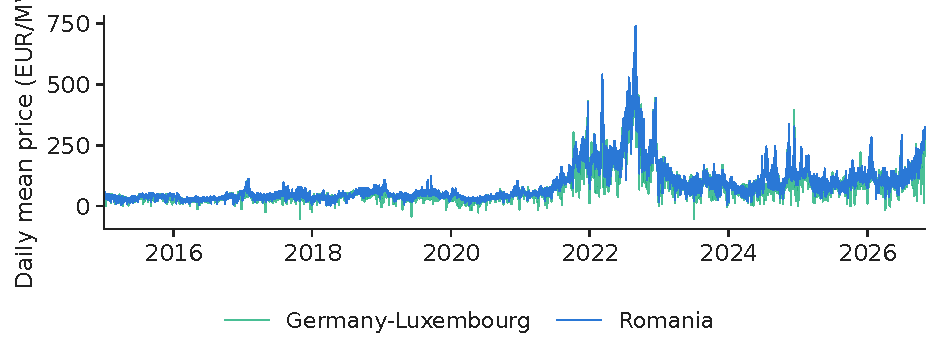
\includegraphics[width=\textwidth,height=0.180\textheight,keepaspectratio]{charts/en/price_history.pdf}\end{center}\vspace{-3mm}
\chartsource{Source: energy-charts.info (Fraunhofer ISE), from exchange and ENTSO-E data. Data: 1 Jan 2015 to 31 Oct 2026, daily means of hourly prices.}
\vspace{0.5mm}
\begin{itemize}\setlength{\itemsep}{0pt}
  \item Mean 2019: 50.41 EUR/MWh
    \begin{itemize}\setlength{\itemsep}{0pt}
      \item Mean 2022: 265.31 EUR/MWh
      \item Highest day 738.28 on 30 Aug 2022
      \item Correlation of daily means RO--DE-LU: 0.94.
    \end{itemize}
\end{itemize}
\par\vfill\manager{choose the training window deliberately: three years, as in Lago et al. (2021), here.}\par\vspace{0.5mm}
\par\vfill\noindent{\scriptsize\color{FooterGray}}\hfill\qlink{NN\_L13\_price\_history}{Quantlets/L13/NN_L13_price_history}\par\vspace{0.5mm}
\end{frame}

\begin{frame}{Solar power has turned the midday peak into a trough}
\small
\intuition{the hourly shape is the strongest regularity a model can learn, and it has changed within six years.}
\vspace{-1mm}\[ \bar P_{\cdot,h}^{(y)}=\frac{1}{|D_y|}\sum_{d\in D_y}P_{d,h} \]\vspace{-2mm}
\begin{center}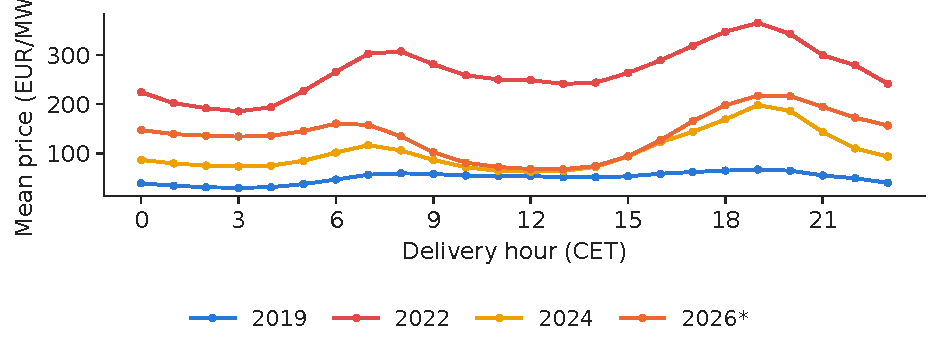
\includegraphics[width=\textwidth,height=0.311\textheight,keepaspectratio]{charts/en/hourly_profile.pdf}\end{center}\vspace{-3mm}
\chartsource{Source: energy-charts.info (Fraunhofer ISE), from exchange and ENTSO-E data. Data: 2019, 2022, 2024 and 2026 (*January-October), Romania.}
\vspace{0.5mm}
\begin{itemize}\setlength{\itemsep}{0pt}
  \item 2026 (January--October): lowest hour 13 at 67.90 EUR/MWh, highest hour 19 at 217.05 EUR/MWh.
\end{itemize}
\par\vfill\manager{a forecaster must predict 24 different hours, not one daily number: hence 24 outputs.}\par\vspace{0.5mm}
\par\vfill\noindent{\scriptsize\color{FooterGray}}\hfill\qlink{NN\_L13\_hourly\_profile}{Quantlets/L13/NN_L13_hourly_profile}\par\vspace{0.5mm}
\end{frame}

\begin{frame}{Information set at gate closure: what the model may use}
\footnotesize
\intuition{a forecast for day $d$ may use only what is known before 12:00 CET on day $d-1$.}
\begin{columns}[T,onlytextwidth]
\begin{column}{0.53\textwidth}
\[ \hat{\mathbf y}_d=f_{\btheta}(\mathbf x_d),\quad \mathbf x_d\in\mathcal I_{d-1} \]\[ \mathbf x_d=(\mathbf y_{d-1},\mathbf y_{d-2},\mathbf y_{d-3},\mathbf y_{d-7},\mathbf y^{\text{DE}}_{d-1},\boldsymbol\ell_{d-2},\mathbf c_d) \]{\footnotesize\begin{itemize}\setlength{\itemsep}{0pt}
  \item \textbf{\txtwhere}
    \begin{itemize}\setlength{\itemsep}{0pt}
      \item $\mathbf y_d\in\R^{24}$ = Romanian prices of day $d$
      \item $\mathbf y^{\text{DE}}$ = DE-LU prices
      \item $\boldsymbol\ell$ = Romanian load (complete two days back)
      \item $\mathbf c_d$ = day-of-week dummies
      \item $\mathcal I_{d-1}$ = information at gate closure.
    \end{itemize}
\end{itemize}\par}
\end{column}
\begin{column}{0.44\textwidth}
\begin{itemize}\setlength{\itemsep}{2pt}
  \item \textbf{151 inputs}, 3\,819 daily samples since 2016.
  \item \textbf{Rolling origin}: re-estimate on the last 1\,092 days, forecast the next day, move one day.
  \item \textbf{Test once}: 364 days never used for fitting or tuning.
\end{itemize}
\end{column}
\end{columns}
\par\vfill\manager{load of day $d-1$ is not complete at noon
    \begin{itemize}\setlength{\itemsep}{0pt}
      \item Using it would leak the future into the forecast.
    \end{itemize}}\par\vspace{0.5mm}
\par\vfill\noindent{\scriptsize\color{FooterGray}}\hfill\tryit{notebook \S1}\par\vspace{0.5mm}
\end{frame}

\begin{frame}{Error measures and the benchmark every model must beat}
\footnotesize
\intuition{report errors in EUR/MWh and relative to the naive forecast, never as a percentage of a price that can be zero.}
\begin{columns}[T,onlytextwidth]
\begin{column}{0.53\textwidth}
\[ \mathrm{MAE}=\frac{1}{24|\mathcal T|}\sum_{d\in\mathcal T}\sum_{h}|y_{d,h}-\hat y_{d,h}|,\quad \mathrm{rMAE}=\frac{\mathrm{MAE}}{\mathrm{MAE}^{\text{naive}}} \]\[ \hat y^{\text{naive}}_{d,h}=\begin{cases}y_{d-7,h}, & \text{Mon, Sat, Sun}\\ y_{d-1,h}, & \text{Tue--Fri}\end{cases} \]{\footnotesize\begin{itemize}\setlength{\itemsep}{0pt}
  \item \textbf{\txtwhere}
    \begin{itemize}\setlength{\itemsep}{0pt}
      \item $\mathcal T$ = test days
      \item $\mathrm{rMAE}<1$ = better than naive
      \item The root mean squared error (RMSE) weights spikes more.
    \end{itemize}
\end{itemize}\par}
\end{column}
\begin{column}{0.44\textwidth}
\begin{itemize}\setlength{\itemsep}{2pt}
  \item \textbf{Test year}: mean 134.59 EUR/MWh, standard deviation 77.19, range \ensuremath{-}97.55 to 954.59
    \begin{itemize}\setlength{\itemsep}{0pt}
      \item 195 negative hours.
    \end{itemize}
  \item \textbf{Naive}: mean absolute error (MAE) 27.74 EUR/MWh.
\end{itemize}
\end{column}
\end{columns}
\par\vfill\manager{a model with rMAE above 1 should not be deployed, however deep.}\par\vspace{0.5mm}
\par\vfill\noindent{\scriptsize\color{FooterGray}}\hfill\tryit{notebook \S1}\par\vspace{0.5mm}
\end{frame}


\section{A strong linear benchmark and a deep network}

\begin{frame}{Variance-stabilising transformation: price spikes and negative prices}
\footnotesize
\intuition{the area hyperbolic sine behaves like a log for large prices and like the identity near zero, so it accepts negative prices.}
\begin{columns}[T,onlytextwidth]
\begin{column}{0.53\textwidth}
\[ z=\asinh\!\Big(\frac{y-\tilde m}{\hat\sigma}\Big),\quad \hat\sigma=\frac{\mathrm{MAD}}{0.6745},\quad y=\tilde m+\hat\sigma\sinh(\hat z) \]{\footnotesize\begin{itemize}\setlength{\itemsep}{0pt}
  \item \textbf{\txtwhere}
    \begin{itemize}\setlength{\itemsep}{0pt}
      \item $\tilde m$ = median of the training window
      \item Median absolute deviation (MAD) scaled to a standard deviation
      \item $\hat z$ = forecast on the transformed scale.
    \end{itemize}
\end{itemize}\par}
\end{column}
\begin{column}{0.44\textwidth}
\begin{itemize}\setlength{\itemsep}{2pt}
  \item \textbf{Fitted on the window only}: no test information enters $\tilde m$, $\hat\sigma$.
  \item \textbf{Same transform for LEAR and the DNN}, so differences come from the model, not from the scale.
\end{itemize}
\end{column}
\end{columns}
\par\vfill\manager{transform before fitting, invert after forecasting, evaluate in EUR/MWh.}\par\vspace{0.5mm}
\par\vfill\noindent{\scriptsize\color{FooterGray}(Uniejewski, Weron \& Ziel, 2018)}\hfill\tryit{notebook \S2}\par\vspace{0.5mm}
\end{frame}

\begin{frame}{LEAR: 24 Lasso regressions, one per hour}
\footnotesize
\intuition{a linear model with many lags, where the Lasso keeps only the lags that matter for each hour.}
\begin{columns}[T,onlytextwidth]
\begin{column}{0.53\textwidth}
\[ \hat{\boldsymbol\beta}_h=\argmin_{\boldsymbol\beta}\sum_{d\in W}\big(z_{d,h}-\mathbf x_d^{\top}\boldsymbol\beta\big)^2+\lambda_h\lVert\boldsymbol\beta\rVert_1 \]{\footnotesize\begin{itemize}\setlength{\itemsep}{0pt}
  \item \textbf{\txtwhere}
    \begin{itemize}\setlength{\itemsep}{0pt}
      \item $W$ = last 1\,092 days
      \item $\lambda_h$ chosen by the Akaike information criterion (AIC) on the Lasso path
      \item Re-estimated every day: 364 $\times$ 24 fits.
    \end{itemize}
\end{itemize}\par}
\end{column}
\begin{column}{0.44\textwidth}
\begin{itemize}\setlength{\itemsep}{2pt}
  \item \textbf{Lasso-estimated autoregressive model (LEAR)}: MAE 22.79 EUR/MWh, rMAE 0.822.
  \item \textbf{Why it is hard to beat}: estimated in seconds, interpretable, adapts every day.
\end{itemize}
\end{column}
\end{columns}
\par\vfill\manager{always report LEAR next to any network: it is the open benchmark of the field.}\par\vspace{0.5mm}
\par\vfill\noindent{\scriptsize\color{FooterGray}(Lago et al., 2021)}\hfill\tryit{notebook \S2}\par\vspace{0.5mm}
\end{frame}

\begin{frame}{The DNN: one network, 24 outputs, trained on the same inputs}
\footnotesize
\intuition{a multilayer perceptron (MLP) forecasts the whole day at once, so hours share what they learn.}
\begin{columns}[T,onlytextwidth]
\begin{column}{0.55\textwidth}
\[ \hat{\mathbf z}_d=\mathbf W_3\,\ReLU\big(\mathbf W_2\,\ReLU(\mathbf W_1\mathbf x_d+\mathbf b_1)+\mathbf b_2\big)+\mathbf b_3 \]\[ \loss=\frac{1}{24|W'|}\sum_{d\in W'}\lVert\mathbf z_d-\hat{\mathbf z}_d\rVert_1,\ \ z_{d,h}=\asinh\frac{y_{d,h}-m_d}{s_d} \]{\footnotesize\begin{itemize}\setlength{\itemsep}{0pt}
  \item \textbf{\txtwhere}
    \begin{itemize}\setlength{\itemsep}{0pt}
      \item $m_d$ = median price of day $d-1$
      \item $s_d$ = MAD of the lagged prices + 1
      \item Rectified linear unit (ReLU)
      \item $W'$ = first 80\,\% of the window.
    \end{itemize}
\end{itemize}\par}
\end{column}
\begin{column}{0.42\textwidth}
\begin{itemize}\setlength{\itemsep}{2pt}
  \item \textbf{Deep neural network (DNN)}: MAE 23.06 EUR/MWh, mean of 4 seeds (single seeds 23.57--24.03).
  \item \textbf{Size}: 256 and 128 units, 74\,904 parameters, dropout 0.1, Adam, early stopping on the last 20\,\%.
  \item \textbf{Per-day scaling} keeps the network usable when the price level jumps.
\end{itemize}
\end{column}
\end{columns}
\par\vfill\manager{average several seeds
    \begin{itemize}\setlength{\itemsep}{0pt}
      \item One seed is one draw of a random estimator.
    \end{itemize}}\par\vspace{0.5mm}
\par\vfill\noindent{\scriptsize\color{FooterGray}(Lago et al., 2021)}\hfill\tryit{notebook \S3}\par\vspace{0.5mm}
\end{frame}

\begin{frame}{Early stopping picks the epoch on data the network did not train on}
\small
\intuition{training loss keeps falling; the validation loss tells when to stop.}
\vspace{-1mm}\[ e^{*}=\argmin_{e}\loss_{\text{val}}(\btheta_e) \]\vspace{-2mm}
\begin{center}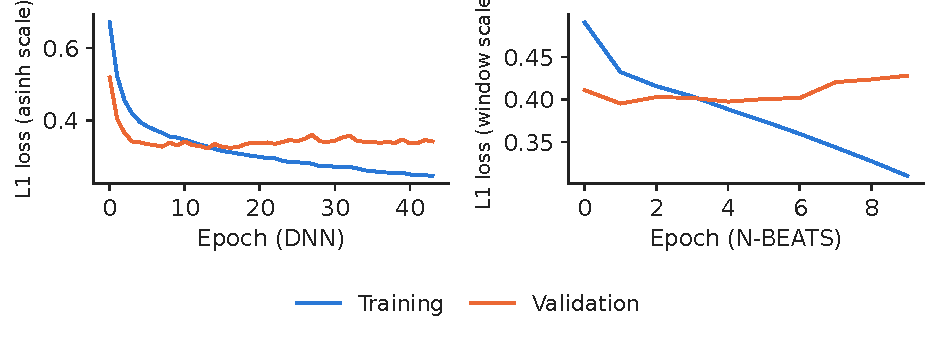
\includegraphics[width=\textwidth,height=0.462\textheight,keepaspectratio]{charts/en/training_curves.pdf}\end{center}\vspace{-3mm}
\chartsource{Source: energy-charts.info (Fraunhofer ISE), from exchange and ENTSO-E data. Data: training windows before 1 Nov 2025, Romania.}
\vspace{0.5mm}
\begin{itemize}\setlength{\itemsep}{0pt}
  \item DNN: best epoch 14 of 44
    \begin{itemize}\setlength{\itemsep}{0pt}
      \item N-BEATS: best epoch 2 of 10 (patience rule).
    \end{itemize}
\end{itemize}
\par\vfill\noindent{\scriptsize\color{FooterGray}}\hfill\qlink{NN\_L13\_training\_curves}{Quantlets/L13/NN_L13_training_curves}\par\vspace{0.5mm}
\end{frame}


\section{Deep forecasting architectures}

\begin{frame}{A probabilistic recurrent network for forecasting}
\footnotesize
\intuition{the recurrent state summarises the past; the network outputs the parameters of tomorrow's distribution.}
\begin{columns}[T,onlytextwidth]
\begin{column}{0.53\textwidth}
\[ \mathbf h_t=\mathrm{LSTM}(\mathbf h_{t-1},y_{t-1},\mathbf c_t),\quad y_t\mid\mathbf h_t\sim\mathcal N\big(\mu(\mathbf h_t),\sigma^2(\mathbf h_t)\big) \]\[ \loss=-\sum_{t}\log p\big(y_t\mid\mu(\mathbf h_t),\sigma(\mathbf h_t)\big) \]{\footnotesize\begin{itemize}\setlength{\itemsep}{0pt}
  \item \textbf{\txtwhere}
    \begin{itemize}\setlength{\itemsep}{0pt}
      \item Long short-term memory network (LSTM, Lecture 5)
      \item $\mathbf c_t$ = covariates
      \item Trained on many related series at once
      \item Multi-step forecasts by sampling $y_t$ and feeding it back.
    \end{itemize}
\end{itemize}\par}
\end{column}
\begin{column}{0.44\textwidth}
\begin{itemize}\setlength{\itemsep}{2pt}
  \item \textbf{Deep autoregressive recurrent network (DeepAR)}: one global model for many series.
  \item \textbf{Its idea lives on} in the foundation models below: global training, probabilistic output.
\end{itemize}
\end{column}
\end{columns}
\par\vfill\manager{useful when you have thousands of related series (stores, meters, assets), not one.}\par\vspace{0.5mm}
\par\vfill\noindent{\scriptsize\color{FooterGray}(Salinas et al., 2020)}\par\vspace{0.5mm}
\end{frame}

\begin{frame}{N-BEATS: stacked blocks that explain the input and forecast the rest}
\footnotesize
\intuition{each block removes what it can explain from the input (backcast) and adds its part to the forecast.}
\begin{columns}[T,onlytextwidth]
\begin{column}{0.53\textwidth}
\[ \mathbf h_\ell=\mathrm{FC}_\ell(\mathbf r_{\ell-1}),\ \ \hat{\mathbf r}_\ell=\mathbf V^{b}_\ell\mathbf h_\ell,\ \ \hat{\mathbf y}_\ell=\mathbf V^{f}_\ell\mathbf h_\ell \]\[ \mathbf r_\ell=\mathbf r_{\ell-1}-\hat{\mathbf r}_\ell,\qquad \hat{\mathbf y}=\sum_{\ell=1}^{L}\hat{\mathbf y}_\ell \]{\footnotesize\begin{itemize}\setlength{\itemsep}{0pt}
  \item \textbf{\txtwhere}
    \begin{itemize}\setlength{\itemsep}{0pt}
      \item $\mathbf r_0$ = last 168 hours, standardised per window
      \item $\mathrm{FC}_\ell$ = 4 layers of width 256
      \item $L$ = 6 blocks
      \item 1\,739\,904 parameters
      \item Output 24 hours.
    \end{itemize}
\end{itemize}\par}
\end{column}
\begin{column}{0.44\textwidth}
\begin{itemize}\setlength{\itemsep}{2pt}
  \item \textbf{Neural basis expansion analysis (N-BEATS)}: prices only, trained once before the test year on every hourly origin.
  \item \textbf{Test MAE} 23.23 EUR/MWh (3 seeds: 23.69 to 24.12).
\end{itemize}
\end{column}
\end{columns}
\par\vfill\manager{a univariate network does not see German prices or load: compare it with LEAR, which does.}\par\vspace{0.5mm}
\par\vfill\noindent{\scriptsize\color{FooterGray}(Oreshkin et al., 2020)}\hfill\tryit{notebook \S3}\par\vspace{0.5mm}
\end{frame}

\begin{frame}{Transformers for time series: patches become tokens}
\footnotesize
\intuition{cut the series into short patches, embed each patch like a word and let attention compare them.}
\begin{columns}[T,onlytextwidth]
\begin{column}{0.53\textwidth}
\[ \mathbf p_j=(y_{(j-1)P+1},\dots,y_{jP}),\quad \mathbf e_j=\mathbf W_{e}\mathbf p_j+\mathbf q_j \]\[ \mathrm{Attn}(\mathbf Q,\mathbf K,\mathbf V)=\softmax\!\Big(\frac{\mathbf Q\mathbf K^{\top}}{\sqrt{d_k}}\Big)\mathbf V \]{\footnotesize\begin{itemize}\setlength{\itemsep}{0pt}
  \item \textbf{\txtwhere}
    \begin{itemize}\setlength{\itemsep}{0pt}
      \item $P$ = patch length (e.g.\ 16 or 32 hours)
      \item $\mathbf q_j$ = position encoding
      \item $\mathbf Q,\mathbf K,\mathbf V$ = projections of $\mathbf e_j$ (Lecture 7).
    \end{itemize}
\end{itemize}\par}
\end{column}
\begin{column}{0.44\textwidth}
\begin{itemize}\setlength{\itemsep}{2pt}
  \item \textbf{Patch time-series transformer (PatchTST)}: 2,048 hours become 128 tokens of 16: attention cost falls 256 times.
  \item \textbf{Foundation models} below use exactly this design, pre-trained on huge collections of series.
\end{itemize}
\end{column}
\end{columns}
\par\vfill\manager{patching is what makes long contexts (weeks of hourly data) affordable.}\par\vspace{0.5mm}
\par\vfill\noindent{\scriptsize\color{FooterGray}(Nie et al., 2023)}\par\vspace{0.5mm}
\end{frame}


\section{Time-series foundation models}

\begin{frame}{A foundation model forecasts a series it has never seen}
\footnotesize
\intuition{one network is pre-trained on many series; at use time it only reads our context, with no gradient step.}
\begin{columns}[T,onlytextwidth]
\begin{column}{0.53\textwidth}
\[ \hat q^{\tau}_{T+k}=g_{\btheta^{*}}\big(y_{T-C+1:T}\big)_{k,\tau} \]\[ \btheta^{*}=\argmin_{\btheta}\sum_{s\in\mathcal S}\sum_{t,\tau}\rho_\tau\big(y^{(s)}_t-\hat q^{\tau,(s)}_t\big) \]{\footnotesize\begin{itemize}\setlength{\itemsep}{0pt}
  \item \textbf{\txtwhere}
    \begin{itemize}\setlength{\itemsep}{0pt}
      \item $\mathcal S$ = pre-training corpus (public and synthetic series)
      \item $C$ = context length (2\,048 hours here)
      \item $\rho_\tau$ = quantile (pinball) loss
      \item $k=1,\dots,24$ = horizon
      \item $\btheta^{*}$ is frozen.
    \end{itemize}
\end{itemize}\par}
\end{column}
\begin{column}{0.44\textwidth}
\begin{itemize}\setlength{\itemsep}{2pt}
  \item \textbf{Three models tested, zero-shot}
    \begin{itemize}\setlength{\itemsep}{0pt}
      \item Chronos-2 (Amazon, 2025): covariates and many series together
      \item Chronos-Bolt base (Amazon): direct quantile forecasts
      \item Time-series Foundation Model (TimesFM) 2.5 (Google): decoder-only
    \end{itemize}
\end{itemize}
\end{column}
\end{columns}
\par\vfill\manager{zero-shot means no training cost and no data pipeline, but also no adaptation to our market.}\par\vspace{0.5mm}
\par\vfill\noindent{\scriptsize\color{FooterGray}(Ansari et al., 2024, 2025; Das et al., 2024)}\hfill\tryit{notebook \S4}\par\vspace{0.5mm}
\end{frame}

\begin{frame}{Chronos: tokenisation of time series}
\footnotesize
\intuition{scale the series, cut its values into bins, and train a language model to predict the next bin.}
\begin{columns}[T,onlytextwidth]
\begin{column}{0.53\textwidth}
\[ \tilde y_t=\frac{y_t}{s},\ \ s=\frac{1}{C}\sum_{t}|y_t|,\qquad v_t=\mathrm{bin}(\tilde y_t)\in\{1,\dots,B\} \]\[ \loss=-\sum_{t}\log p_{\btheta}(v_{t+1}\mid v_{1:t}) \]{\footnotesize\begin{itemize}\setlength{\itemsep}{0pt}
  \item \textbf{\txtwhere}
    \begin{itemize}\setlength{\itemsep}{0pt}
      \item $s$ = mean absolute scale of the context
      \item $B$ = 4,096 bins in the original Chronos
      \item The model is a T5 language model
      \item Chronos-Bolt and Chronos-2 replace the bins by patches and quantile heads.
    \end{itemize}
\end{itemize}\par}
\end{column}
\begin{column}{0.44\textwidth}
\begin{itemize}\setlength{\itemsep}{2pt}
  \item \textbf{Scaling makes series comparable}: a price in EUR/MWh and a sales count become the same kind of input.
  \item \textbf{Quantile loss} gives probabilistic forecasts directly (next section).
\end{itemize}
\end{column}
\end{columns}
\par\vfill\manager{the model knows shapes (seasonality, mean reversion), not the Romanian market.}\par\vspace{0.5mm}
\par\vfill\noindent{\scriptsize\color{FooterGray}(Ansari et al., 2024)}\par\vspace{0.5mm}
\end{frame}

\begin{frame}{Test-year accuracy: all nine forecasts on the same days}
\small
\begin{columns}[T,onlytextwidth]
\begin{column}{0.52\textwidth}
{\footnotesize\renewcommand{\arraystretch}{1.05}\setlength{\tabcolsep}{4pt}
\begin{tabular}{@{}lrrr@{}}\toprule
Model & MAE & RMSE & rMAE \\ \midrule
\textbf{Chronos-2 with covariates} & \cellcolor{Forest!55}20.41 & 33.88 & \cellcolor{Forest!55}0.736 \\
Chronos-2 & \cellcolor{Forest!50}20.72 & 34.23 & \cellcolor{Forest!50}0.747 \\
the ensemble & \cellcolor{Forest!50}20.77 & 34.27 & \cellcolor{Forest!49}0.749 \\
Chronos-Bolt & \cellcolor{Forest!36}21.67 & 34.51 & \cellcolor{Forest!36}0.781 \\
TimesFM & \cellcolor{Forest!26}22.37 & 36.08 & \cellcolor{Forest!26}0.806 \\
LEAR & \cellcolor{Forest!19}22.79 & 36.27 & \cellcolor{Forest!19}0.822 \\
DNN & \cellcolor{Forest!15}23.06 & 38.42 & \cellcolor{Forest!15}0.831 \\
N-BEATS & \cellcolor{Forest!13}23.23 & 36.64 & \cellcolor{Forest!13}0.837 \\
the naive benchmark & \cellcolor{Crimson!55}27.74 & 44.57 & \cellcolor{Crimson!55}1.000 \\
\bottomrule\end{tabular}}
\end{column}
\begin{column}{0.45\textwidth}
\begin{itemize}\setlength{\itemsep}{3pt}
  \item \textbf{Lowest MAE}: Chronos-2 with covariates, 20.41 EUR/MWh.
  \item \textbf{Best foundation model}: Chronos-2 with covariates, 20.41, better than LEAR (22.79) without any training on our data.
  \item \textbf{All models} beat the naive forecast: rMAE below 1.
  \item Green = lower error
    \begin{itemize}\setlength{\itemsep}{0pt}
      \item Significance on the next slides.
    \end{itemize}
\end{itemize}
\end{column}
\end{columns}
\par\vfill\noindent{\scriptsize\color{FooterGray}(own computation, EUR/MWh)}\hfill\tryit{notebook \S4}\par\vspace{0.5mm}
\end{frame}

\begin{frame}{Trained networks versus zero-shot foundation models}
\small
\intuition{the same 8\,736 hours, the same information set, nine forecasting strategies.}
\begin{center}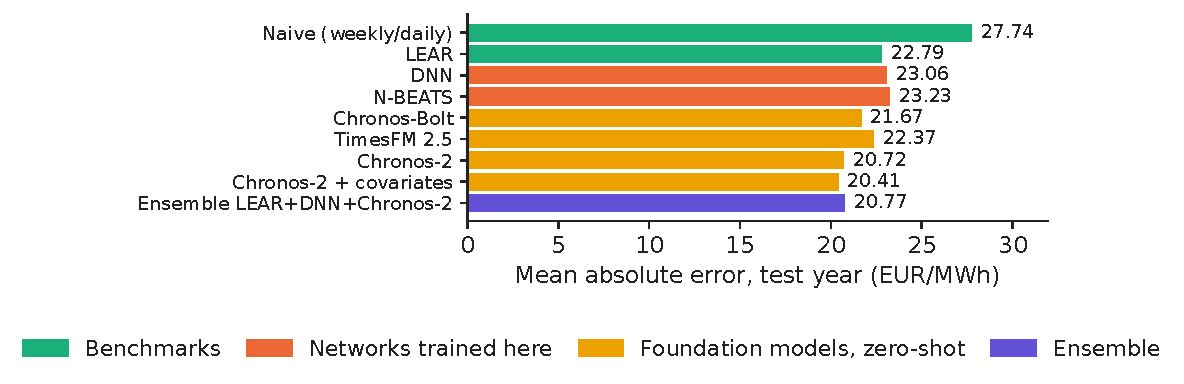
\includegraphics[width=\textwidth,height=0.480\textheight,keepaspectratio]{charts/en/mae_models.pdf}\end{center}\vspace{-3mm}
\chartsource{Source: energy-charts.info (Fraunhofer ISE), from exchange and ENTSO-E data. Data: 1 Nov 2025 to 31 Oct 2026, 360 days x 24 hours, Romania.}
\vspace{0.5mm}
\begin{itemize}\setlength{\itemsep}{0pt}
  \item Ensemble = simple mean of LEAR, DNN and Chronos-2: MAE 20.77 EUR/MWh.
\end{itemize}
\par\vfill\manager{start with the benchmark and a foundation model: both cost minutes, not weeks.}\par\vspace{0.5mm}
\par\vfill\noindent{\scriptsize\color{FooterGray}}\hfill\qlink{NN\_L13\_mae\_models}{Quantlets/L13/NN_L13_mae_models}\par\vspace{0.5mm}
\end{frame}

\begin{frame}{Errors are largest in the evening and around solar hours}
\small
\intuition{the average hides hours where all models struggle together.}
\vspace{-1mm}\[ \mathrm{MAE}_h=\frac{1}{|\mathcal T|}\sum_{d\in\mathcal T}|y_{d,h}-\hat y_{d,h}| \]\vspace{-2mm}
\begin{center}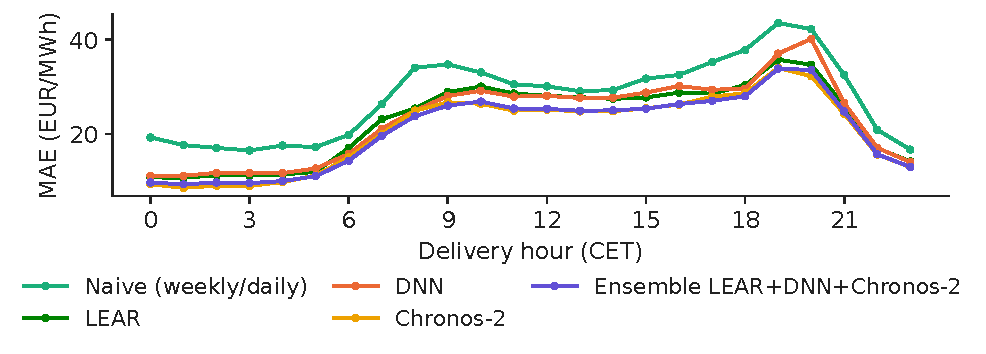
\includegraphics[width=\textwidth,height=0.440\textheight,keepaspectratio]{charts/en/mae_by_hour.pdf}\end{center}\vspace{-3mm}
\chartsource{Source: energy-charts.info (Fraunhofer ISE), from exchange and ENTSO-E data. Data: 1 Nov 2025 to 31 Oct 2026, 360 days x 24 hours, Romania.}
\vspace{0.5mm}
\begin{itemize}\setlength{\itemsep}{0pt}
  \item LEAR: worst hour 19 (35.78), best hour 1 (10.75)
    \begin{itemize}\setlength{\itemsep}{0pt}
      \item Chronos-2: worst hour 19 (34.05).
    \end{itemize}
\end{itemize}
\par\vfill\noindent{\scriptsize\color{FooterGray}}\hfill\qlink{NN\_L13\_mae\_by\_hour}{Quantlets/L13/NN_L13_mae_by_hour}\par\vspace{0.5mm}
\end{frame}

\begin{frame}{Forecasts for one week of the test year}
\small
\intuition{all three models follow the daily shape; none of them anticipates the largest evening spikes in full.}
\begin{center}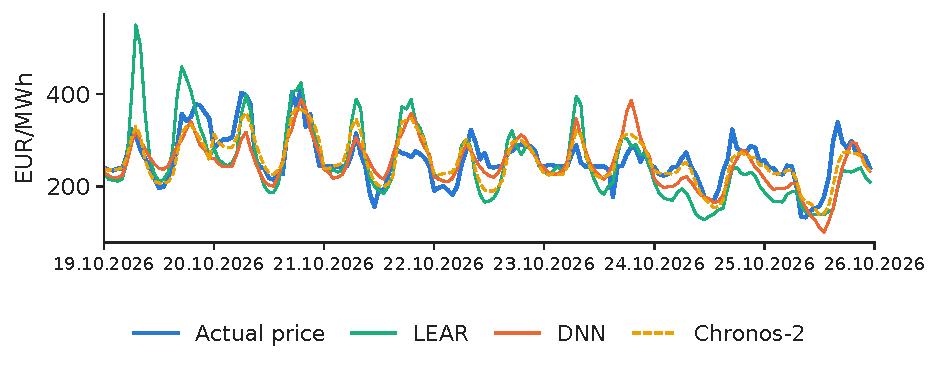
\includegraphics[width=\textwidth,height=0.513\textheight,keepaspectratio]{charts/en/forecast_week.pdf}\end{center}\vspace{-3mm}
\chartsource{Source: energy-charts.info (Fraunhofer ISE), from exchange and ENTSO-E data. Data: 19 Oct 2026 to 25 Oct 2026, hourly, Romania.}
\vspace{0.5mm}
\begin{itemize}\setlength{\itemsep}{0pt}
  \item Week 19 Oct 2026 to 25 Oct 2026: MAE LEAR 43.34, DNN 32.33, Chronos-2 25.41 EUR/MWh.
\end{itemize}
\par\vfill\noindent{\scriptsize\color{FooterGray}}\hfill\qlink{NN\_L13\_forecast\_week}{Quantlets/L13/NN_L13_forecast_week}\par\vspace{0.5mm}
\end{frame}

\begin{frame}{Longer context helps the foundation model, up to a point}
\small
\intuition{the model sees only the context: one week shows the daily shape, three months also the level.}
\begin{center}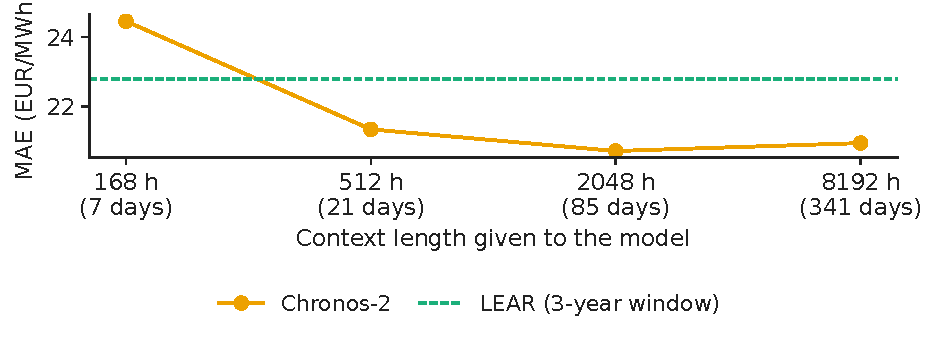
\includegraphics[width=\textwidth,height=0.431\textheight,keepaspectratio]{charts/en/context_length.pdf}\end{center}\vspace{-3mm}
\chartsource{Source: energy-charts.info (Fraunhofer ISE), from exchange and ENTSO-E data. Data: 1 Nov 2025 to 31 Oct 2026, 360 days x 24 hours, Romania.}
\vspace{0.5mm}
\begin{itemize}\setlength{\itemsep}{0pt}
  \item Chronos-2 MAE: 168 h 24.45, 512 h 21.34, 2,048 h 20.72, 8,192 h 20.95 EUR/MWh.
\end{itemize}
\par\vfill\manager{the context length is the main tuning knob of a zero-shot model: choose it on past data.}\par\vspace{0.5mm}
\par\vfill\noindent{\scriptsize\color{FooterGray}}\hfill\qlink{NN\_L13\_context\_length}{Quantlets/L13/NN_L13_context_length}\par\vspace{0.5mm}
\end{frame}

\begin{frame}{Covariates in a foundation model: German prices and Romanian load}
\footnotesize
\intuition{Chronos-2 reads several aligned series and lets attention share information across them.}
\begin{columns}[T,onlytextwidth]
\begin{column}{0.53\textwidth}
\[ \hat{\mathbf q}_{T+1:T+24}=g_{\btheta^{*}}\big(y_{1:T},\ x^{\text{DE}}_{1:T},\ x^{\text{HU}}_{1:T},\ \ell_{1:T}\big) \]{\footnotesize\begin{itemize}\setlength{\itemsep}{0pt}
  \item \textbf{\txtwhere}
    \begin{itemize}\setlength{\itemsep}{0pt}
      \item Past-only covariates: DE-LU and HU prices and Romanian load up to the forecast origin (their future values are not known at gate closure).
    \end{itemize}
\end{itemize}\par}
\end{column}
\begin{column}{0.44\textwidth}
\begin{itemize}\setlength{\itemsep}{2pt}
  \item \textbf{Without covariates}: MAE 20.72
    \begin{itemize}\setlength{\itemsep}{0pt}
      \item \textbf{with covariates}: 20.41 EUR/MWh.
    \end{itemize}
  \item \textbf{Covariates helped} here
    \begin{itemize}\setlength{\itemsep}{0pt}
      \item Test, do not assume.
    \end{itemize}
\end{itemize}
\end{column}
\end{columns}
\par\vfill\manager{a covariate known in advance (a weather or load forecast) is worth more than one known only in the past.}\par\vspace{0.5mm}
\par\vfill\noindent{\scriptsize\color{FooterGray}(Ansari et al., 2025)}\hfill\tryit{notebook \S5}\par\vspace{0.5mm}
\end{frame}

\begin{frame}{Is the difference real? The Diebold--Mariano test on daily losses}
\footnotesize
\intuition{a lower average error can be luck; test whether the daily loss differential has mean zero.}
\begin{columns}[T,onlytextwidth]
\begin{column}{0.53\textwidth}
\[ \Delta_d=\lVert\mathbf e^{A}_d\rVert_1-\lVert\mathbf e^{B}_d\rVert_1,\qquad \mathrm{DM}=\frac{\bar\Delta}{\hat\sigma_\Delta/\sqrt{|\mathcal T|}}\ \overset{a}{\sim}\ \mathcal N(0,1) \]{\footnotesize\begin{itemize}\setlength{\itemsep}{0pt}
  \item \textbf{\txtwhere}
    \begin{itemize}\setlength{\itemsep}{0pt}
      \item $\mathbf e^{A}_d\in\R^{24}$ = errors of model A on day $d$
      \item One statistic per pair (multivariate version)
      \item One-sided $H_1$: B is more accurate than A
      \item $|\mathcal T|$ = 360 days.
    \end{itemize}
\end{itemize}\par}
\end{column}
\begin{column}{0.44\textwidth}
\begin{itemize}\setlength{\itemsep}{2pt}
  \item \textbf{Diebold--Mariano (DM)}: LEAR vs DNN, $p$ = 0.761
    \begin{itemize}\setlength{\itemsep}{0pt}
      \item LEAR vs Chronos-2, $p$ = $<$0.001.
    \end{itemize}
  \item \textbf{Daily, not hourly}: hours of one day share the same information, so they are not independent.
\end{itemize}
\end{column}
\end{columns}
\par\vfill\manager{claim that a model is better only with a test on the test period.}\par\vspace{0.5mm}
\par\vfill\noindent{\scriptsize\color{FooterGray}(Diebold \& Mariano, 1995; Ziel \& Weron, 2018)}\hfill\tryit{notebook \S6}\par\vspace{0.5mm}
\end{frame}

\begin{frame}{Pairwise Diebold--Mariano tests for all models}
\small
\intuition{green cells: the column model is significantly more accurate than the row model.}
\begin{center}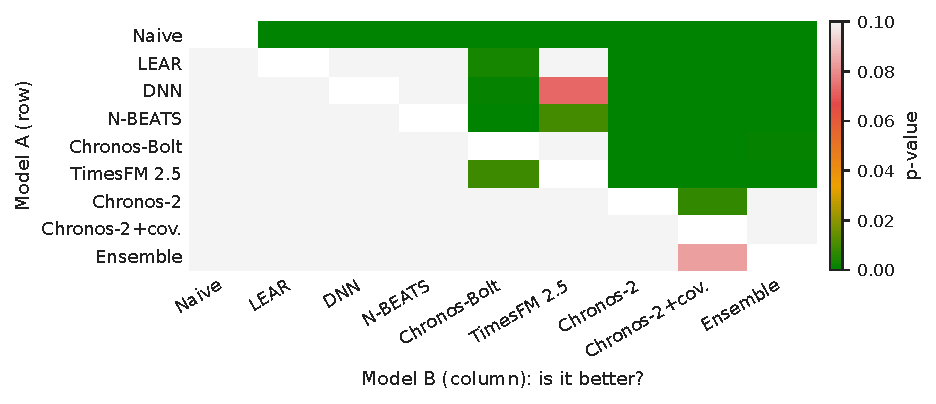
\includegraphics[width=\textwidth,height=0.534\textheight,keepaspectratio]{charts/en/dm_pvalues.pdf}\end{center}\vspace{-3mm}
\chartsource{Source: energy-charts.info (Fraunhofer ISE), from exchange and ENTSO-E data. Data: 1 Nov 2025 to 31 Oct 2026, 360 days x 24 hours, Romania.}
\vspace{0.5mm}
\begin{itemize}\setlength{\itemsep}{0pt}
  \item Ensemble vs LEAR: $p$ = $<$0.001
    \begin{itemize}\setlength{\itemsep}{0pt}
      \item Ensemble vs Chronos-2: $p$ = 0.565.
    \end{itemize}
\end{itemize}
\par\vfill\noindent{\scriptsize\color{FooterGray}}\hfill\qlink{NN\_L13\_dm\_pvalues}{Quantlets/L13/NN_L13_dm_pvalues}\par\vspace{0.5mm}
\end{frame}


\section{Probabilistic forecasts and conformal calibration}

\begin{frame}{Quantile forecasts are scored with the pinball loss}
\footnotesize
\intuition{a quantile forecast is good when the right share of outcomes falls below it and the band is narrow.}
\begin{columns}[T,onlytextwidth]
\begin{column}{0.53\textwidth}
\[ \rho_\tau(u)=u\,\big(\tau-\mathbb 1\{u<0\}\big),\quad u=y-\hat q^{\tau} \]\[ \mathrm{PL}=\frac{1}{9}\sum_{\tau\in\{0.1,\dots,0.9\}}\frac{1}{24|\mathcal T|}\sum_{d,h}\rho_\tau\big(y_{d,h}-\hat q^{\tau}_{d,h}\big) \]{\footnotesize\begin{itemize}\setlength{\itemsep}{0pt}
  \item \textbf{\txtwhere}
    \begin{itemize}\setlength{\itemsep}{0pt}
      \item $\tau$ = quantile level
      \item The average over the nine deciles approximates the continuous ranked probability score.
    \end{itemize}
\end{itemize}\par}
\end{column}
\begin{column}{0.44\textwidth}
\begin{itemize}\setlength{\itemsep}{2pt}
  \item \textbf{Average pinball loss, test year} (EUR/MWh)
    \begin{itemize}\setlength{\itemsep}{0pt}
      \item Chronos-2 8.25; with covariates 8.11
      \item Chronos-Bolt 8.62; TimesFM 8.97
      \item LEAR + empirical errors of the last 60 days 9.12
    \end{itemize}
\end{itemize}
\end{column}
\end{columns}
\par\vfill\manager{a battery or a risk desk needs quantiles
    \begin{itemize}\setlength{\itemsep}{0pt}
      \item Score them with pinball, not with MAE.
    \end{itemize}}\par\vspace{0.5mm}
\par\vfill\noindent{\scriptsize\color{FooterGray}}\hfill\tryit{notebook \S7}\par\vspace{0.5mm}
\end{frame}

\begin{frame}{A week of Chronos-2 quantiles: the band widens where prices jump}
\small
\intuition{the model is less sure in the evening hours, exactly where the errors are largest.}
\begin{center}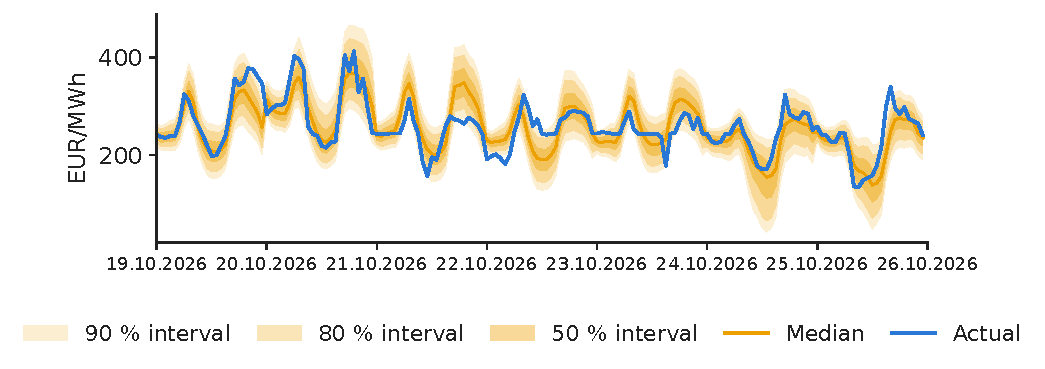
\includegraphics[width=\textwidth,height=0.600\textheight,keepaspectratio]{charts/en/chronos_fan.pdf}\end{center}\vspace{-3mm}
\chartsource{Source: energy-charts.info (Fraunhofer ISE), from exchange and ENTSO-E data. Data: 19 Oct 2026 to 25 Oct 2026, hourly, Romania.}
\par\vfill\noindent{\scriptsize\color{FooterGray}}\hfill\qlink{NN\_L13\_chronos\_fan}{Quantlets/L13/NN_L13_chronos_fan}\par\vspace{0.5mm}
\end{frame}

\begin{frame}{Split-conformal correction of prediction intervals}
\footnotesize
\intuition{measure how far the outcomes fell outside the raw band in the recent past, and widen (or shrink) the band by that amount.}
\begin{columns}[T,onlytextwidth]
\begin{column}{0.53\textwidth}
\[ s_i=\max\big(\hat q^{\alpha/2}_i-y_i,\ y_i-\hat q^{1-\alpha/2}_i\big),\quad \hat Q=s_{(\lceil (n+1)(1-\alpha)\rceil)} \]\[ \hat C_{d,h}=\big[\hat q^{\alpha/2}_{d,h}-\hat Q,\ \hat q^{1-\alpha/2}_{d,h}+\hat Q\big],\qquad \Pr\big(y\in\hat C\big)\ge 1-\alpha \]{\footnotesize\begin{itemize}\setlength{\itemsep}{0pt}
  \item \textbf{\txtwhere}
    \begin{itemize}\setlength{\itemsep}{0pt}
      \item $s_i$ = conformity scores on the last 60 days ($n$ = 24 $\times$ days)
      \item $s_{(k)}$ = $k$-th smallest
      \item The guarantee holds under exchangeability, only approximately for time series.
    \end{itemize}
\end{itemize}\par}
\end{column}
\begin{column}{0.44\textwidth}
\begin{itemize}\setlength{\itemsep}{2pt}
  \item \textbf{Conformalised quantile regression (CQR)} applied to Chronos-2, 80\,\% band: raw coverage 76.5\,\%, corrected 79.3\,\%.
  \item \textbf{Width}: 60.03 $\rightarrow$ 63.89 EUR/MWh.
\end{itemize}
\end{column}
\end{columns}
\par\vfill\manager{a foundation model plus conformal calibration is a cheap, honest probabilistic forecaster.}\par\vspace{0.5mm}
\par\vfill\noindent{\scriptsize\color{FooterGray}(Romano, Patterson \& Candès, 2019)}\hfill\tryit{notebook \S7}\par\vspace{0.5mm}
\end{frame}

\begin{frame}{Conformal calibration moves coverage towards the nominal level}
\small
\intuition{black lines: the nominal level; bars: the share of test hours inside the band.}
\begin{center}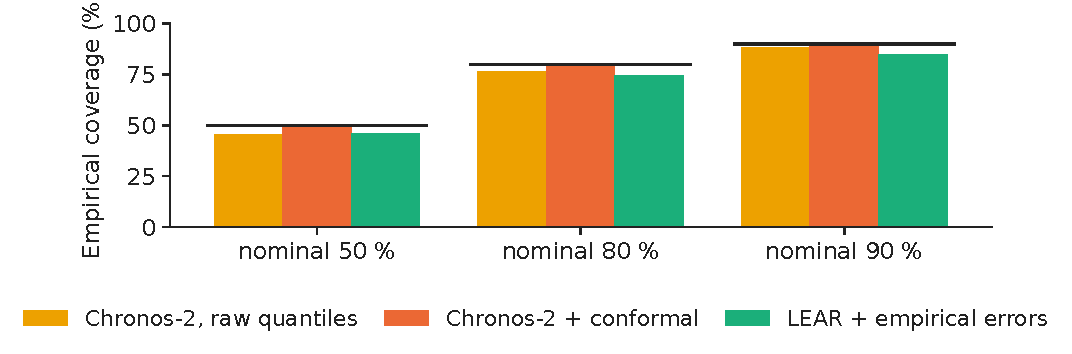
\includegraphics[width=\textwidth,height=0.520\textheight,keepaspectratio]{charts/en/coverage.pdf}\end{center}\vspace{-3mm}
\chartsource{Source: energy-charts.info (Fraunhofer ISE), from exchange and ENTSO-E data. Data: 1 Nov 2025 to 31 Oct 2026, 360 days x 24 hours, Romania.}
\vspace{0.5mm}
\begin{itemize}\setlength{\itemsep}{0pt}
  \item 90\,\% band: raw 88.3\,\%, conformal 89.4\,\%, LEAR + empirical errors 85.0\,\%
    \begin{itemize}\setlength{\itemsep}{0pt}
      \item TimesFM 80\,\%: raw 79.6\,\%, conformal 79.7\,\%.
    \end{itemize}
\end{itemize}
\par\vfill\noindent{\scriptsize\color{FooterGray}}\hfill\qlink{NN\_L13\_coverage}{Quantlets/L13/NN_L13_coverage}\par\vspace{0.5mm}
\end{frame}

\begin{frame}{Load is easier than price: foundation models forecast it within a few percent}
\small
\intuition{load is smooth and seasonal, the shapes a pre-trained model knows best.}
\vspace{-1mm}\[ \mathrm{MAPE}=\frac{100}{24|\mathcal T|}\sum_{d,h}\Big|\frac{\ell_{d,h}-\hat\ell_{d,h}}{\ell_{d,h}}\Big| \]\vspace{-2mm}
\begin{center}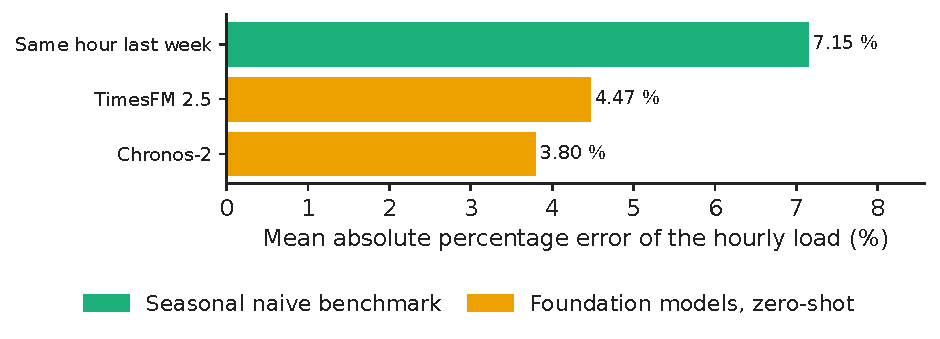
\includegraphics[width=\textwidth,height=0.319\textheight,keepaspectratio]{charts/en/load_mape.pdf}\end{center}\vspace{-3mm}
\chartsource{Source: energy-charts.info (Fraunhofer ISE), from exchange and ENTSO-E data. Data: 1 Nov 2025 to 31 Oct 2026, 360 days, Romanian load.}
\vspace{0.5mm}
\begin{itemize}\setlength{\itemsep}{0pt}
  \item Mean absolute percentage error (MAPE): last week 7.15\,\%, TimesFM 4.47\,\%, Chronos-2 3.80\,\% (MAE 214.4 MW, mean load 5\,932 MW).
\end{itemize}
\par\vfill\manager{percentage errors are fine for load, which is never close to zero.}\par\vspace{0.5mm}
\par\vfill\noindent{\scriptsize\color{FooterGray}}\hfill\qlink{NN\_L13\_load\_mape}{Quantlets/L13/NN_L13_load_mape}\par\vspace{0.5mm}
\end{frame}


\section{Foundation models for financial risk}

\begin{frame}{Value-at-Risk is a conditional quantile, backtested by counting violations}
\footnotesize
\intuition{a 1\,\% VaR should be breached on about 1\,\% of days, and the breaches should not cluster.}
\begin{columns}[T,onlytextwidth]
\begin{column}{0.53\textwidth}
\[ \Pr\big(r_{t+1}<\mathrm{VaR}^{\alpha}_{t+1}\mid\mathcal F_t\big)=\alpha,\qquad I_{t+1}=\mathbb 1\{r_{t+1}<\mathrm{VaR}^{\alpha}_{t+1}\} \]\[ \mathrm{LR}_{uc}=-2\ln\frac{(1-\alpha)^{n_0}\alpha^{n_1}}{(1-\hat\pi)^{n_0}\hat\pi^{n_1}}\sim\chi^2_1 \]{\footnotesize\begin{itemize}\setlength{\itemsep}{0pt}
  \item \textbf{\txtwhere}
    \begin{itemize}\setlength{\itemsep}{0pt}
      \item $r_t$ = daily log return (\%)
      \item $n_1$ = violations, $n_0$ = other days, $\hat\pi=n_1/(n_0+n_1)$
      \item Likelihood ratio (LR) test of Kupiec
      \item Christoffersen adds a test of independence of $I_t$.
    \end{itemize}
\end{itemize}\par}
\end{column}
\begin{column}{0.44\textwidth}
\begin{itemize}\setlength{\itemsep}{2pt}
  \item \textbf{Three forecasters}
    \begin{itemize}\setlength{\itemsep}{0pt}
      \item Historical simulation (HS): empirical quantile of the last 250 days
      \item Generalised autoregressive conditional heteroskedasticity (GARCH): GARCH(1,1) with Student-$t$ errors, re-estimated every 21 days
      \item Chronos-2 quantiles from the last 1,024 returns, zero-shot
    \end{itemize}
\end{itemize}
\end{column}
\end{columns}
\par\vfill\manager{the Basel traffic light turns on the number of 1\,\% exceptions in 250 days.}\par\vspace{0.5mm}
\par\vfill\noindent{\scriptsize\color{FooterGray}(Kupiec, 1995; Christoffersen, 1998)}\hfill\tryit{notebook \S9}\par\vspace{0.5mm}
\end{frame}

\begin{frame}{A one-sided conformal shift turns a raw quantile into a calibrated VaR}
\footnotesize
\intuition{if the model's quantile was breached too often in the last year, lower it by exactly the amount that would have fixed it.}
\begin{columns}[T,onlytextwidth]
\begin{column}{0.53\textwidth}
\[ s_i=\hat q^{\alpha}_i-r_i,\qquad c_t=s_{(\lceil (n+1)(1-\alpha)\rceil)}\ \text{over the last } n=250 \]\[ \widehat{\mathrm{VaR}}^{\alpha}_{t+1}=\hat q^{\alpha}_{t+1}-c_t \]{\footnotesize\begin{itemize}\setlength{\itemsep}{0pt}
  \item \textbf{\txtwhere}
    \begin{itemize}\setlength{\itemsep}{0pt}
      \item $\hat q^{\alpha}$ = raw Chronos-2 quantile
      \item $c_t>0$ widens the VaR, $c_t<0$ narrows it
      \item The shift uses only past forecasts and returns.
    \end{itemize}
\end{itemize}\par}
\end{column}
\begin{column}{0.44\textwidth}
\begin{itemize}\setlength{\itemsep}{2pt}
  \item \textbf{S\&P 500, 1\,\% level}: raw Chronos-2 22 violations, conformal 16, expected 17.2.
  \item \textbf{Same idea} as the energy bands, applied to one tail.
\end{itemize}
\end{column}
\end{columns}
\par\vfill\manager{recalibration is a model change: document it and backtest it out of sample.}\par\vspace{0.5mm}
\par\vfill\noindent{\scriptsize\color{FooterGray}(Romano et al., 2019)}\hfill\tryit{notebook \S9}\par\vspace{0.5mm}
\end{frame}

\begin{frame}{S\&P 500: the calibrated foundation-model VaR follows volatility regimes}
\small
\intuition{both lines widen in March 2020 and in April 2025; red dots are the days the conformal Chronos-2 VaR was breached.}
\begin{center}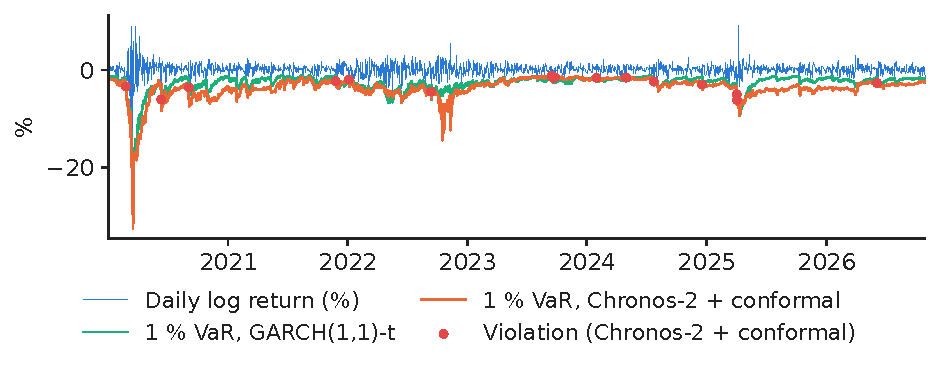
\includegraphics[width=\textwidth,height=0.600\textheight,keepaspectratio]{charts/en/var_sp500.pdf}\end{center}\vspace{-3mm}
\chartsource{Source: Yahoo Finance, daily quotes. Data: 2 Jan 2020 to 30 Oct 2026, trading days, S\&P 500.}
\par\vfill\noindent{\scriptsize\color{FooterGray}}\hfill\qlink{NN\_L13\_var\_sp500}{Quantlets/L13/NN_L13_var_sp500}\par\vspace{0.5mm}
\end{frame}

\begin{frame}{Backtests, January 2020 to October 2026: S\&P 500 and Bitcoin}
\small
{\scriptsize\renewcommand{\arraystretch}{1.05}\setlength{\tabcolsep}{4pt}
\begin{tabular}{@{}llrrrrrr@{}}\toprule
Asset & Model & Viol.\ 1\,\% & $p_{uc}$ & $p_{ind}$ & Viol.\ 5\,\% & $p_{uc}$ & Tick loss 5\,\% \\ \midrule
S\&P 500 & HS (250 days) & 31 & \cellcolor{Crimson!52}0.003 & 0.002 & 89 & \cellcolor{Forest!55}0.729 & 0.1582 \\
 & GARCH(1,1)-$t$ & 32 & \cellcolor{Crimson!54}0.001 & 0.607 & 132 & \cellcolor{Crimson!55}0.000 & 0.1347 \\
 & Chronos-2, raw & 22 & \cellcolor{Forest!55}0.262 & 0.285 & 122 & \cellcolor{Crimson!55}0.000 & 0.1368 \\
 & Chronos-2 + conformal & 16 & \cellcolor{Forest!55}0.774 & 0.138 & 93 & \cellcolor{Forest!55}0.434 & 0.1383 \\
Bitcoin & HS (250 days) & 33 & \cellcolor{Forest!55}0.123 & 0.458 & 126 & \cellcolor{Forest!55}0.912 & 0.3633 \\
 & GARCH(1,1)-$t$ & 22 & \cellcolor{Forest!55}0.543 & 0.189 & 128 & \cellcolor{Forest!55}0.770 & 0.3587 \\
 & Chronos-2, raw & 31 & \cellcolor{Forest!55}0.242 & 0.402 & 134 & \cellcolor{Forest!55}0.404 & 0.3591 \\
 & Chronos-2 + conformal & 21 & \cellcolor{Forest!55}0.413 & 0.170 & 120 & \cellcolor{Forest!55}0.657 & 0.3614 \\
\bottomrule\end{tabular}}
\par\vspace{0.5mm}{\scriptsize \begin{itemize}\setlength{\itemsep}{0pt}
  \item Expected violations: S\&P 500 17.2 (1\,\%) and 85.9 (5\,\%) over 1\,717 days; Bitcoin 25.0 and 124.8 over 2\,496 days (traded every day).
  \item Green $p$-value: coverage not rejected at 10\,\%; red: rejected. Tick loss = pinball loss at $\tau=0.05$ (lower is better).
\end{itemize}}
\par\vfill\noindent{\scriptsize\color{FooterGray}(own computation; Kupiec, 1995; Christoffersen, 1998)}\hfill\tryit{notebook \S9}\par\vspace{0.5mm}
\end{frame}

\begin{frame}{Quantile forecasts from language models and time-series models}
\small
\begin{itemize}\setlength{\itemsep}{3pt}
  \item \textbf{Large language model (LLM) route} (Lecture 12)
    \begin{itemize}\setlength{\itemsep}{0pt}
      \item The returns are written as text in a prompt; a general model answers with a number
      \item LLM-VaR and, for the expected shortfall (ES), LLM-ES, of our group: zero-shot, no fine-tuning (Pele et al., 2026)
    \end{itemize}
  \item \textbf{Time-series foundation model route} (this lecture)
    \begin{itemize}\setlength{\itemsep}{0pt}
      \item Numbers enter as scaled patches; the output is a set of quantiles
      \item Cheaper per forecast, can be run locally, calibrated here with a conformal shift
    \end{itemize}
  \item \textbf{Common rules}
    \begin{itemize}\setlength{\itemsep}{0pt}
      \item Backtest out of sample, count violations, test independence, compare with GARCH and HS
    \end{itemize}
\end{itemize}
\end{frame}

\section*{Wrap-up}

\begin{frame}{Quiz 1: leakage}
\small
\begin{itemize}
  \item A colleague adds the actual Romanian load of day $d$ to the inputs of the price forecast for day $d$ and the MAE falls
    \begin{itemize}\setlength{\itemsep}{0pt}
      \item Should you deploy the model?
    \end{itemize}
\end{itemize}
\vspace{2mm}
\begin{exampleblock}{Answer}
\begin{itemize}
  \item No: the actual load of day $d$ is unknown at 12:00 on $d-1$
    \begin{itemize}\setlength{\itemsep}{0pt}
      \item Use the operator's load forecast or lags available at gate closure.
    \end{itemize}
\end{itemize}
\end{exampleblock}
\end{frame}

\begin{frame}{Quiz 2: conformal width}
\small
\begin{itemize}
  \item The raw 80\,\% Chronos-2 band covered 76.5\,\% of test hours
    \begin{itemize}\setlength{\itemsep}{0pt}
      \item What does the conformal step do to its width, and why?
    \end{itemize}
\end{itemize}
\vspace{2mm}
\begin{exampleblock}{Answer}
\begin{itemize}
  \item It changes it by $\hat Q$, the $(1-\alpha)$ quantile of recent out-of-band distances: wider if the band was too narrow, narrower if too wide (here 60.03 $\rightarrow$ 63.89 EUR/MWh).
\end{itemize}
\end{exampleblock}
\end{frame}

\begin{frame}{Quiz 3: Kupiec}
\small
\begin{itemize}
  \item Over 1\,717 days a 1\,\% VaR had 3 times the expected number of violations
    \begin{itemize}\setlength{\itemsep}{0pt}
      \item Is the Kupiec $p$-value large or small?
    \end{itemize}
\end{itemize}
\vspace{2mm}
\begin{exampleblock}{Answer}
\begin{itemize}
  \item Small: $\hat\pi$ is far from $\alpha$, so $\mathrm{LR}_{uc}$ is large and coverage is rejected
    \begin{itemize}\setlength{\itemsep}{0pt}
      \item The model underestimates risk.
    \end{itemize}
\end{itemize}
\end{exampleblock}
\end{frame}

\begin{frame}{Wrap-up}
\small
\begin{itemize}\setlength{\itemsep}{4pt}
  \item Benchmarks first: naive 27.74, LEAR 22.79 EUR/MWh
    \begin{itemize}\setlength{\itemsep}{0pt}
      \item Lowest MAE: Chronos-2 with covariates (20.41).
    \end{itemize}
  \item Foundation models forecast prices and load zero-shot
    \begin{itemize}\setlength{\itemsep}{0pt}
      \item The context length and covariates are their tuning knobs.
    \end{itemize}
  \item Significance by Diebold--Mariano on daily losses
    \begin{itemize}\setlength{\itemsep}{0pt}
      \item Several seeds for every network.
    \end{itemize}
  \item Conformal calibration turns raw quantiles into honest bands and VaR
    \begin{itemize}\setlength{\itemsep}{0pt}
      \item Backtest with Kupiec and Christoffersen.
    \end{itemize}
  \item Next: multimodal models and the synthesis of the course (Lecture 14).
\end{itemize}
\end{frame}

\begin{frame}{Research from our group}
\footnotesize
\begin{itemize}\setlength{\itemsep}{3pt}
  \item \textbf{Four generations of energy price forecasting}: econometric models, machine learning, LSTM and transformers compared on European energy markets, with pre-training and transfer learning (Andrei, Velev, Toma, Pele \& Lessmann, 2024, arXiv 2411.03372).
  \item \textbf{Early warning of price spikes}: explainable gradient boosting on Romanian hourly data
    \begin{itemize}\setlength{\itemsep}{0pt}
      \item The residual load forecast is the main trigger of spike warnings (Andrei, Pele, Cramer, Amza \& Diaconu, 2026, PICBE).
    \end{itemize}
  \item \textbf{Multi-horizon explainability}: which drivers matter from 0--6 hours to two weeks ahead and in which price regime, Romania 2018--2024 (Andrei, Pele \& Cramer, 2026, PICBE).
  \item \textbf{LLM-VaR and LLM-ES}: general-purpose language models produce Value-at-Risk and expected shortfall (ES) forecasts zero-shot from a prompt with past returns (Pele et al., 2026, Expert Systems with Applications).
  \item \textbf{Early warning for crypto `zombies'}: machine learning predicts which crypto-assets will become inactive (Będowska-Sójka, Wójcik \& Pele, 2026, North American Journal of Economics and Finance).
\end{itemize}
\par\vspace{0.5mm}{\scriptsize \begin{itemize}\setlength{\itemsep}{0pt}
  \item Findings as stated in the papers' abstracts; numbers on the other slides come from our own data.
\end{itemize}}
\par\vfill\noindent{\scriptsize\color{FooterGray}(Bucharest University of Economic Studies, ASE; Romanian Academy, Institute for Economic Forecasting, IPE)}\par\vspace{0.5mm}
\end{frame}

\begin{frame}{Want to learn more?}
\small
\begin{columns}[T,onlytextwidth]
\begin{column}{0.5\textwidth}
\begin{itemize}\setlength{\itemsep}{4pt}
  \item \textbf{Chronos} code and models: \href{https://github.com/amazon-science/chronos-forecasting}{github.com/amazon-science/chronos-forecasting}.
  \item \textbf{TimesFM}: \href{https://github.com/google-research/timesfm}{github.com/google-research/timesfm}.
  \item \textbf{epftoolbox}, the open benchmark of Lago et al.\ (2021): \href{https://github.com/jeslago/epftoolbox}{github.com/jeslago/epftoolbox}.
\end{itemize}
\end{column}
\begin{column}{0.47\textwidth}
\begin{itemize}\setlength{\itemsep}{4pt}
  \item \textbf{Conformal prediction}, a gentle introduction: \href{https://arxiv.org/abs/2107.07511}{arXiv:2107.07511}.
  \item \textbf{Forecasting: Principles and Practice}, 3rd ed.: \href{https://otexts.com/fpp3/}{otexts.com/fpp3}.
  \item \textbf{This lecture}: notebook, seminar and Quantlets --- \href{https://github.com/danpele/NEURAL_BIZ}{github.com/danpele/NEURAL\_BIZ}.
\end{itemize}
\end{column}
\end{columns}
\end{frame}

\begin{frame}{References (1/2)}
\scriptsize
\begin{itemize}\setlength{\itemsep}{0pt}\scriptsize
\item Andrei, A.-V., Pele, D.-T., Cramer, A.-A., Amza, A.\ \& Diaconu, D.\ (2026). Explainable AI-based early warning system for electricity price spikes: Evidence from the Romanian market. \textit{Proceedings of the International Conference on Business Excellence}, 20(1), 4820--4836. \href{https://doi.org/10.2478/picbe-2026-0352}{doi:10.2478/picbe-2026-0352}
\item Andrei, A.-V., Pele, D.-T.\ \& Cramer, A.-A.\ (2026). Multi-horizon explainability in energy price forecasting: Disentangling market dynamics and renewable intermittency in Romania's liberalized electricity market. \textit{Proceedings of the International Conference on Business Excellence}, 20(1), 104--117. \href{https://doi.org/10.2478/picbe-2026-0014}{doi:10.2478/picbe-2026-0014}
\item Andrei, A.-V., Velev, G., Toma, F.-M., Pele, D.\,T.\ \& Lessmann, S.\ (2024). Energy price modelling: A comparative evaluation of four generations of forecasting methods. \href{https://arxiv.org/abs/2411.03372}{arXiv:2411.03372}
\item Ansari, A.\,F.\ et al.\ (2024). Chronos: Learning the language of time series. \textit{Transactions on Machine Learning Research}. \href{https://arxiv.org/abs/2403.07815}{arXiv:2403.07815}
\item Ansari, A.\,F.\ et al.\ (2025). Chronos-2: From univariate to universal forecasting. \href{https://arxiv.org/abs/2510.15821}{arXiv:2510.15821}
\item Będowska-Sójka, B., Wójcik, P.\ \& Pele, D.\,T.\ (2026). Early warning systems for cryptocurrency markets: Predicting `zombie' assets using machine learning. \textit{The North American Journal of Economics and Finance}, 81, 102543. \href{https://doi.org/10.1016/j.najef.2025.102543}{doi:10.1016/j.najef.2025.102543}
\item Christoffersen, P.\,F.\ (1998). Evaluating interval forecasts. \textit{International Economic Review}, 39(4), 841--862. \href{https://doi.org/10.2307/2527341}{doi:10.2307/2527341}
\item Das, A., Kong, W., Sen, R.\ \& Zhou, Y.\ (2024). A decoder-only foundation model for time-series forecasting. \textit{Proceedings of the 41st International Conference on Machine Learning}. \href{https://arxiv.org/abs/2310.10688}{arXiv:2310.10688}
\item Diebold, F.\,X.\ \& Mariano, R.\,S.\ (1995). Comparing predictive accuracy. \textit{Journal of Business \& Economic Statistics}, 13(3), 253--263. \href{https://doi.org/10.1080/07350015.1995.10524599}{doi:10.1080/07350015.1995.10524599}
\item Kupiec, P.\,H.\ (1995). Techniques for verifying the accuracy of risk measurement models. \textit{The Journal of Derivatives}, 3(2), 73--84. \href{https://doi.org/10.3905/jod.1995.407942}{doi:10.3905/jod.1995.407942}
\end{itemize}
\end{frame}

\begin{frame}{References (2/2)}
\scriptsize
\begin{itemize}\setlength{\itemsep}{0pt}\scriptsize
\item Lago, J., Marcjasz, G., De Schutter, B.\ \& Weron, R.\ (2021). Forecasting day-ahead electricity prices: A review of state-of-the-art algorithms, best practices and an open-access benchmark. \textit{Applied Energy}, 293, 116983. \href{https://doi.org/10.1016/j.apenergy.2021.116983}{doi:10.1016/j.apenergy.2021.116983}
\item Nie, Y., Nguyen, N.\,H., Sinthong, P.\ \& Kalagnanam, J.\ (2023). A time series is worth 64 words: Long-term forecasting with transformers. \textit{International Conference on Learning Representations}. \href{https://arxiv.org/abs/2211.14730}{arXiv:2211.14730}
\item Oreshkin, B.\,N., Carpov, D., Chapados, N.\ \& Bengio, Y.\ (2020). N-BEATS: Neural basis expansion analysis for interpretable time series forecasting. \textit{International Conference on Learning Representations}. \href{https://arxiv.org/abs/1905.10437}{arXiv:1905.10437}
\item Pele, D.\,T., Bolovăneanu, V., Lin, M.-B., Ren, R., Ginavar, A.\,T., Spilak, B., Andrei, A.-V., Toma, F.-M., Lessmann, S.\ \& Härdle, W.\,K.\ (2026). In the beginning was the Word: LLM-VaR and LLM-ES. \textit{Expert Systems with Applications}, 295, 128676. \href{https://doi.org/10.1016/j.eswa.2025.128676}{doi:10.1016/j.eswa.2025.128676}
\item Romano, Y., Patterson, E.\ \& Candès, E.\ (2019). Conformalized quantile regression. \textit{Advances in Neural Information Processing Systems}, 32. \href{https://arxiv.org/abs/1905.03222}{arXiv:1905.03222}
\item Salinas, D., Flunkert, V., Gasthaus, J.\ \& Januschowski, T.\ (2020). DeepAR: Probabilistic forecasting with autoregressive recurrent networks. \textit{International Journal of Forecasting}, 36(3), 1181--1191. \href{https://doi.org/10.1016/j.ijforecast.2019.07.001}{doi:10.1016/j.ijforecast.2019.07.001}
\item Uniejewski, B., Weron, R.\ \& Ziel, F.\ (2018). Variance stabilizing transformations for electricity spot price forecasting. \textit{IEEE Transactions on Power Systems}, 33(2), 2219--2229. \href{https://doi.org/10.1109/TPWRS.2017.2734563}{doi:10.1109/TPWRS.2017.2734563}
\item Weron, R.\ (2014). Electricity price forecasting: A review of the state-of-the-art with a look into the future. \textit{International Journal of Forecasting}, 30(4), 1030--1081. \href{https://doi.org/10.1016/j.ijforecast.2014.08.008}{doi:10.1016/j.ijforecast.2014.08.008}
\item Ziel, F.\ \& Weron, R.\ (2018). Day-ahead electricity price forecasting with high-dimensional structures: Univariate vs.\ multivariate modeling frameworks. \textit{Energy Economics}, 70, 396--420. \href{https://doi.org/10.1016/j.eneco.2017.12.016}{doi:10.1016/j.eneco.2017.12.016}
\end{itemize}
\end{frame}

\appendix

\section*{Appendix}

\begin{frame}{Appendix A: why the conformal band covers}
\small
\begin{itemize}\setlength{\itemsep}{4pt}
  \item Let $s_1,\dots,s_n,s_{n+1}$ be exchangeable conformity scores
    \begin{itemize}\setlength{\itemsep}{0pt}
      \item The rank of $s_{n+1}$ among them is uniform on $\{1,\dots,n+1\}$.
    \end{itemize}
  \item Hence $\Pr(s_{n+1}\le s_{(k)})\ge k/(n+1)$
    \begin{itemize}\setlength{\itemsep}{0pt}
      \item Choosing $k=\lceil (n+1)(1-\alpha)\rceil$ gives $\Pr(s_{n+1}\le\hat Q)\ge 1-\alpha$.
    \end{itemize}
  \item $s_{n+1}\le\hat Q$ is equivalent to $y_{n+1}\in[\hat q^{\alpha/2}-\hat Q,\hat q^{1-\alpha/2}+\hat Q]$, which is the band.
  \item Hours of a price series are dependent and drift
    \begin{itemize}\setlength{\itemsep}{0pt}
      \item The rolling window of 60 days trades exactness for adaptation.
    \end{itemize}
\end{itemize}
\par\vfill\noindent{\scriptsize\color{FooterGray}(Romano, Patterson \& Candès, 2019)}\par\vspace{0.5mm}
\end{frame}

\begin{frame}{Appendix B: Christoffersen's test of independence}
\small
\begin{itemize}\setlength{\itemsep}{4pt}
  \item Count transitions of the hit sequence: $n_{ij}$ = number of days with $I_{t-1}=i$ and $I_t=j$
    \begin{itemize}\setlength{\itemsep}{0pt}
      \item $\hat\pi_{01}=n_{01}/(n_{00}+n_{01})$, $\hat\pi_{11}=n_{11}/(n_{10}+n_{11})$.
    \end{itemize}
  \item $\mathrm{LR}_{ind}=-2\ln\frac{(1-\hat\pi)^{n_{00}+n_{10}}\hat\pi^{n_{01}+n_{11}}}{(1-\hat\pi_{01})^{n_{00}}\hat\pi_{01}^{n_{01}}(1-\hat\pi_{11})^{n_{10}}\hat\pi_{11}^{n_{11}}}\sim\chi^2_1$.
  \item A small $p$-value means violations cluster: the model reacts too slowly to a volatility shock.
\end{itemize}
\par\vfill\noindent{\scriptsize\color{FooterGray}(Christoffersen, 1998)}\par\vspace{0.5mm}
\end{frame}

\begin{frame}{Appendix C: implementation details}
\small
\begin{itemize}\setlength{\itemsep}{4pt}
  \item LEAR: scikit-learn LassoLarsIC (criterion AIC), standardised inputs, daily re-estimation on 1\,092 days.
  \item DNN and N-BEATS: PyTorch, L1 loss, Adam, early stopping
    \begin{itemize}\setlength{\itemsep}{0pt}
      \item Seeds 20261108 and the next ones.
    \end{itemize}
  \item Foundation models: amazon/chronos-2, amazon/chronos-bolt-base, google/timesfm-2.5-200m-pytorch from Hugging Face, inference only
    \begin{itemize}\setlength{\itemsep}{0pt}
      \item The full run took 2.7 minutes on a laptop.
    \end{itemize}
  \item Hours on the CET calendar
    \begin{itemize}\setlength{\itemsep}{0pt}
      \item The doubled autumn hour is averaged
      \item Days with a missing hour are excluded from training targets and from the test.
    \end{itemize}
\end{itemize}
\end{frame}

\end{document}
